%%%%%%%%%%%%%%%%%%%%%%%%%%%%%%%%%%%%%%%%%
% Lachaise Assignment
% LaTeX Template
% Version 1.0 (26/6/2018)
%
% This template originates from:
% http://www.LaTeXTemplates.com
%
% Authors:
% Marion Lachaise & François Févotte
% Vel (vel@LaTeXTemplates.com)
%
% License:
% CC BY-NC-SA 3.0 (http://creativecommons.org/licenses/by-nc-sa/3.0/)
% 
%%%%%%%%%%%%%%%%%%%%%%%%%%%%%%%%%%%%%%%%%

%----------------------------------------------------------------------------------------
%	PACKAGES AND OTHER DOCUMENT CONFIGURATIONS
%----------------------------------------------------------------------------------------

\documentclass{article}
\bibliographystyle{IEEEtran}
\usepackage[utf8]{inputenc}
\usepackage[english]{babel}
\usepackage{graphicx}
\usepackage[parfill]{parskip}
%%%%%%%%%%%%%%%%%%%%%%%%%%%%%%%%%%%%%%%%%
% Lachaise Assignment
% Structure Specification File
% Version 1.0 (26/6/2018)
%
% This template originates from:
% http://www.LaTeXTemplates.com
%
% Authors:
% Marion Lachaise & François Févotte
% Vel (vel@LaTeXTemplates.com)
%
% License:
% CC BY-NC-SA 3.0 (http://creativecommons.org/licenses/by-nc-sa/3.0/)
% 
%%%%%%%%%%%%%%%%%%%%%%%%%%%%%%%%%%%%%%%%%

%----------------------------------------------------------------------------------------
%	PACKAGES AND OTHER DOCUMENT CONFIGURATIONS
%----------------------------------------------------------------------------------------

\usepackage{amsmath,amsfonts,stmaryrd,amssymb} % Math packages

\usepackage{enumerate} % Custom item numbers for enumerations

\usepackage[ruled]{algorithm2e} % Algorithms

\usepackage[framemethod=tikz]{mdframed} % Allows defining custom boxed/framed environments

\usepackage{listings} % File listings, with syntax highlighting
\lstset{
	basicstyle=\ttfamily, % Typeset listings in monospace font
}

%----------------------------------------------------------------------------------------
%	DOCUMENT MARGINS
%----------------------------------------------------------------------------------------

\usepackage{geometry} % Required for adjusting page dimensions and margins

\geometry{
	paper=a4paper, % Paper size, change to letterpaper for US letter size
	top=2.5cm, % Top margin
	bottom=3cm, % Bottom margin
	left=2.5cm, % Left margin
	right=2.5cm, % Right margin
	headheight=14pt, % Header height
	footskip=1.5cm, % Space from the bottom margin to the baseline of the footer
	headsep=1.2cm, % Space from the top margin to the baseline of the header
	%showframe, % Uncomment to show how the type block is set on the page
}

%----------------------------------------------------------------------------------------
%	FONTS
%----------------------------------------------------------------------------------------

\usepackage[utf8]{inputenc} % Required for inputting international characters
\usepackage[T1]{fontenc} % Output font encoding for international characters

\usepackage{XCharter} % Use the XCharter fonts

%----------------------------------------------------------------------------------------
%	COMMAND LINE ENVIRONMENT
%----------------------------------------------------------------------------------------

% Usage:
% \begin{commandline}
%	\begin{verbatim}
%		$ ls
%		
%		Applications	Desktop	...
%	\end{verbatim}
% \end{commandline}

\mdfdefinestyle{commandline}{
	leftmargin=10pt,
	rightmargin=10pt,
	innerleftmargin=15pt,
	middlelinecolor=black!50!white,
	middlelinewidth=2pt,
	frametitlerule=false,
	backgroundcolor=black!5!white,
	frametitle={Command Line},
	frametitlefont={\normalfont\sffamily\color{white}\hspace{-1em}},
	frametitlebackgroundcolor=black!50!white,
	nobreak,
}

% Define a custom environment for command-line snapshots
\newenvironment{commandline}{
	\medskip
	\begin{mdframed}[style=commandline]
}{
	\end{mdframed}
	\medskip
}

%----------------------------------------------------------------------------------------
%	FILE CONTENTS ENVIRONMENT
%----------------------------------------------------------------------------------------

% Usage:
% \begin{file}[optional filename, defaults to "File"]
%	File contents, for example, with a listings environment
% \end{file}

\mdfdefinestyle{file}{
	innertopmargin=1.6\baselineskip,
	innerbottommargin=0.8\baselineskip,
	topline=false, bottomline=false,
	leftline=false, rightline=false,
	leftmargin=1cm,
	rightmargin=1cm,
	singleextra={%
		\draw[fill=black!10!white](P)++(0,-1.2em)rectangle(P-|O);
		\node[anchor=north west]
		at(P-|O){\ttfamily\mdfilename};
		%
		\def\l{3em}
		\draw(O-|P)++(-\l,0)--++(\l,\l)--(P)--(P-|O)--(O)--cycle;
		\draw(O-|P)++(-\l,0)--++(0,\l)--++(\l,0);
	},
	nobreak,
}

% Define a custom environment for file contents
\newenvironment{file}[1][File]{ % Set the default filename to "File"
	\medskip
	\newcommand{\mdfilename}{#1}
	\begin{mdframed}[style=file]
}{
	\end{mdframed}
	\medskip
}

%----------------------------------------------------------------------------------------
%	NUMBERED QUESTIONS ENVIRONMENT
%----------------------------------------------------------------------------------------

% Usage:
% \begin{question}[optional title]
%	Question contents
% \end{question}

\mdfdefinestyle{question}{
	innertopmargin=1.2\baselineskip,
	innerbottommargin=0.8\baselineskip,
	roundcorner=5pt,
	nobreak,
	singleextra={%
		\draw(P-|O)node[xshift=1em,anchor=west,fill=white,draw,rounded corners=5pt]{%
		Question \theQuestion\questionTitle};
	},
}

\newcounter{Question} % Stores the current question number that gets iterated with each new question

% Define a custom environment for numbered questions
\newenvironment{question}[1][\unskip]{
	\bigskip
	\stepcounter{Question}
	\newcommand{\questionTitle}{~#1}
	\begin{mdframed}[style=question]
}{
	\end{mdframed}
	\medskip
}

%----------------------------------------------------------------------------------------
%	WARNING TEXT ENVIRONMENT
%----------------------------------------------------------------------------------------

% Usage:
% \begin{warn}[optional title, defaults to "Warning:"]
%	Contents
% \end{warn}

\mdfdefinestyle{warning}{
	topline=false, bottomline=false,
	leftline=false, rightline=false,
	nobreak,
	singleextra={%
		\draw(P-|O)++(-0.5em,0)node(tmp1){};
		\draw(P-|O)++(0.5em,0)node(tmp2){};
		\fill[black,rotate around={45:(P-|O)}](tmp1)rectangle(tmp2);
		\node at(P-|O){\color{white}\scriptsize\bf !};
		\draw[very thick](P-|O)++(0,-1em)--(O);%--(O-|P);
	}
}

% Define a custom environment for warning text
\newenvironment{warn}[1][Warning:]{ % Set the default warning to "Warning:"
	\medskip
	\begin{mdframed}[style=warning]
		\noindent{\textbf{#1}}
}{
	\end{mdframed}
}

%----------------------------------------------------------------------------------------
%	INFORMATION ENVIRONMENT
%----------------------------------------------------------------------------------------

% Usage:
% \begin{info}[optional title, defaults to "Info:"]
% 	contents
% 	\end{info}

\mdfdefinestyle{info}{%
	topline=false, bottomline=false,
	leftline=false, rightline=false,
	nobreak,
	singleextra={%
		\fill[black](P-|O)circle[radius=0.4em];
		\node at(P-|O){\color{white}\scriptsize\bf i};
		\draw[very thick](P-|O)++(0,-0.8em)--(O);%--(O-|P);
	}
}

% Define a custom environment for information
\newenvironment{info}[1][Info:]{ % Set the default title to "Info:"
	\medskip
	\begin{mdframed}[style=info]
		\noindent{\textbf{#1}}
}{
	\end{mdframed}
}


%----------------------------------------------------------------------------------------
%	ASSIGNMENT INFORMATION
%----------------------------------------------------------------------------------------

\title{Cluster and Cloud Computing Assignment 2
		\\ City Analytic on the Cloud} % Title of the assignment

\author{ Zhaofeng Qiu \texttt{1101584}
        \\ Aoqi Zuo \texttt{1028089}
        \\Rongbing Shan \texttt{945388}
        \\Tingli Qiu \texttt{990497}
        \\Yawei Sun \texttt{....}}% Author name and email address

%\date{University of Melbourne --- \today} % University, school and/or department name(s) and a date

%----------------------------------------------------------------------------------------

\begin{document}

\maketitle % Print the title

%----------------------------------------------------------------------------------------
%	INTRODUCTION
%----------------------------------------------------------------------------------------
\begin{abstract}
This paper is a summary on the group project of COMP90024 Cluster and Cloud Computing at the University of Melbourne 2020 Semester 1, conducted by group \#17. The use of social media has been increasing rapidly in past years, as a result, many useful information can now be provided by such social media, like Twitter. A cloud-based solution is introduced in the project to collect and analyze tweets from Australia based on 
six different scenarios, with parallel comparison with other Australian data gathered from \textit{AURIN}. The results are visualized on a web portal for better illustration. The cloud-based system is deployed to Melbourne Research Cloud using software configuration management tool \textit{ANSIBLE} and docker technologies. 
\end{abstract}

\section{Introduction}
Social media has become an essential part of people’s daily life. The usage of Facebook, Twitter, Instagram and other social networks have been growing tremendously during the past decade. Taking Twitter for an example, based on statistics \textit{from Internet Live Stats}\footnote{https://www.internetlivestats.com}, twitter now has over 330 million monthly users and there are over 500 million tweets sent each day. People nowadays share their activities, opinions, feelings and knowledge through social media, thus making the data valuable and informative. Despite the rich information given by the tremendous number of data, such large data volume also causes challenges for the analyzing system, since systems performance may drop heavily and failure rate arises with traditional methods. Therefore, high performance computing and cloud-based solutions come into our sight to harvest the informative big data from twitter, with good performance as well as improved disaster recovery and scalability.

In this project, we will develop an integrated cloud based system with the functionality of collecting tweets from twitter, managing the large-volume data in NOSQL database, analyzing the tweets data with comparison to AURIN statistics and visualizing the result on a web page. We have divided the system into several major function parts: Tweet Harvesters, Database, Tweet Analyzer, Backend and Frontend, and they will be discussed in detail in coming sections. Multiple technologies are used in this project. The major functioning body of the system was developed with Python and Java and would be deployed to Melbourne Research Cloud (NeCTAR Research Cloud) with Ansible. CouchDB has been used as a centralized database for data storage in a cluster mode. Also, docker technologies are taken for simple deployment and better program management. 

In this report, we will introduce the design and architecture of our system, and go through each major functioning part. Besides, the five analytics scenarios we have developed from tweets data will be explained in detail. Also, we will address the challenges met during both the development and deployment phase of the project and discuss the error handling capability of the system. \\
\newline
\begin{itemize}
	\item The scripts of our project can be accessed on github repository: 
	\begin{itemize}
		\item https://github.com/CCC-2020-G17/city-analytics-on-the-cloud
	\end{itemize}

	\item And there is a video demonstration on the whole system through:
	\begin{itemize}
		\item https://www.youtube.com/watch?v=LYTV-1LKQMo\&feature=youtu.be
	\end{itemize}
	
	\item The webpage can be accessed (with Unimelb VPN) through:
	\begin{itemize}
		\item http://172.26.132.125
	\end{itemize}
\end{itemize}


\section{System Design and Architecture}
\label{sec:systemDesignAndArchitecture}
The architecture of our system is well designed. It is aimed to provide both a beautiful front-end web application and a RESTFul API server with high availability, high scalability, and fault tolerance. The overall architecture is shown in Figure \ref{fig:systemArchitecture}. 

\begin{figure}[htp]
\centering
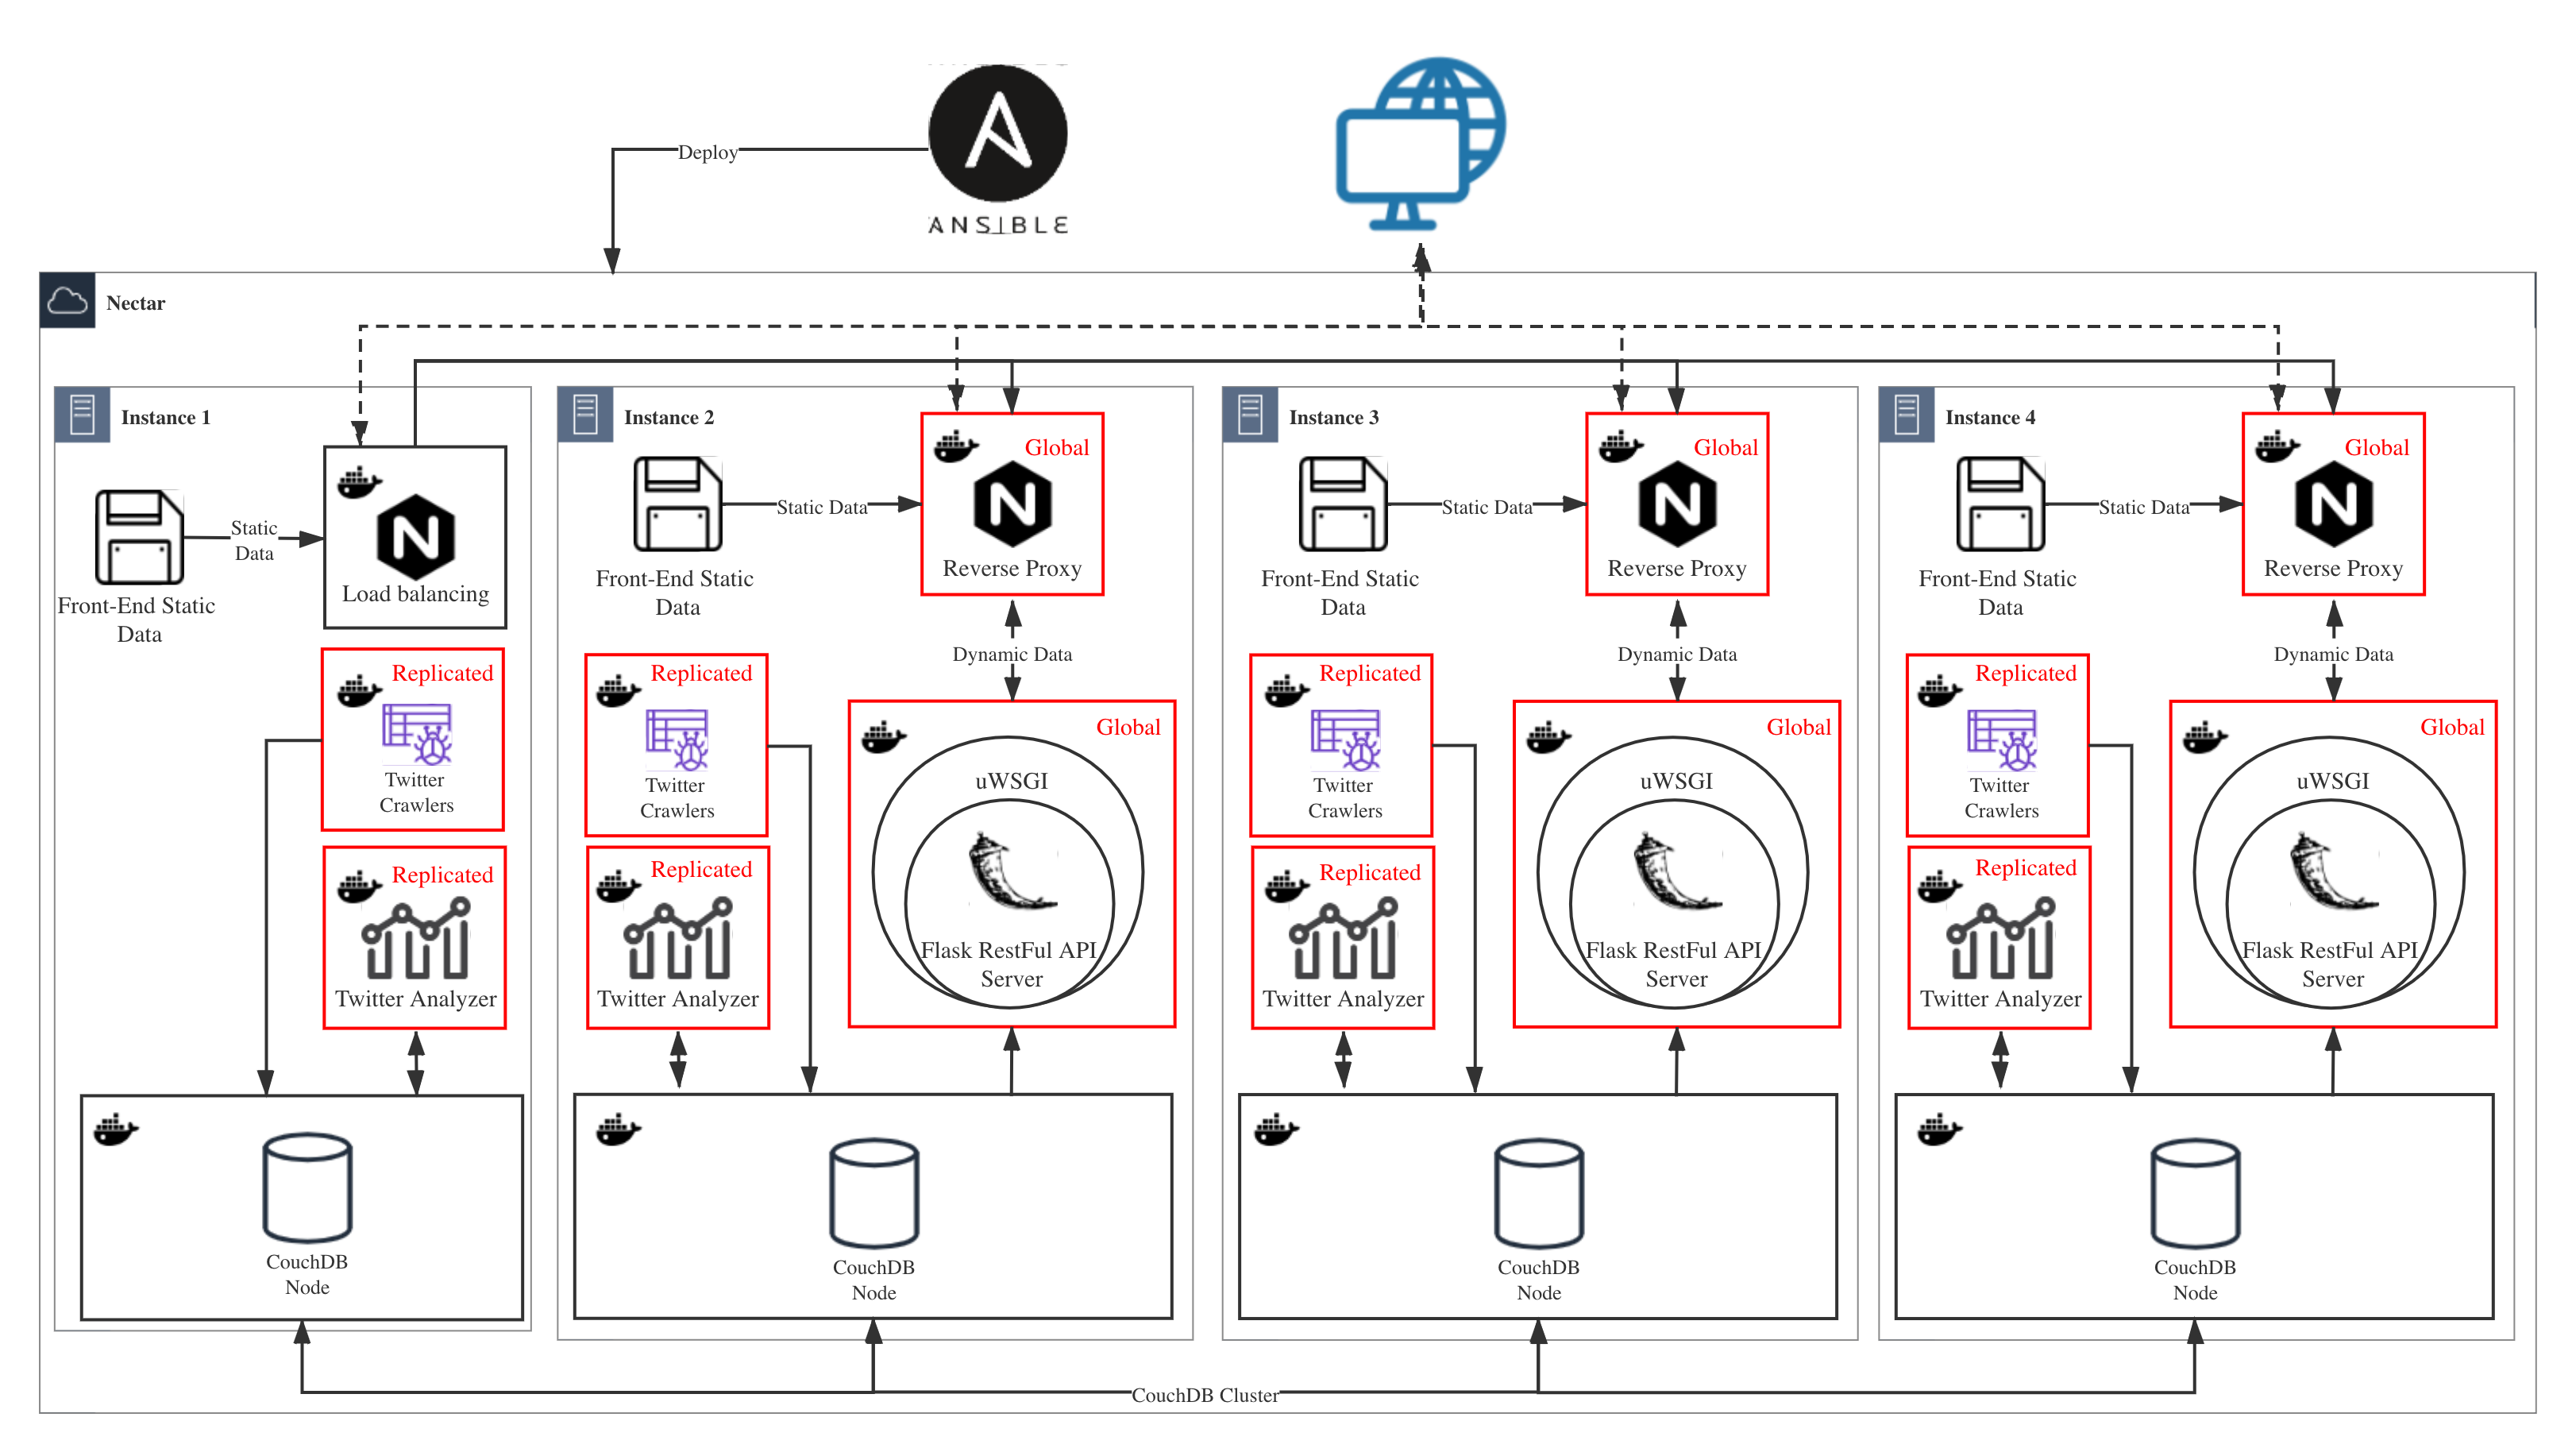
\includegraphics[width=\textwidth]{img/architecture.png}
\caption{System Architecture}
\label{fig:systemArchitecture}
\end{figure}

\subsection{Availability}
We continue to optimize our architecture through in-depth thinking and repeated practice to improve the availability of our system with limited resources.

Firstly, we run an \textit{Nginx} server in our first instance to provide Load balancing. For requests that need to access the dynamic data in our database, it would pass the request to the other three servers averagely. In this way, we can efficiently distribute the incoming network traffic to our backend servers in the cluster. When it comes to the situation where the first instance may crash, users can still access our application through the IPs of the other three nodes. However, this solution is not good enough and is contradict to high availability. We had tried to use two \textit{Nginx} server with a software called Keepalived to provide a more fault-tolerant system. However, we found out that we are not allowed to use floating IP in \textit{Nectar}. Since we cannot set a virtual IP for our \textit{Nginx} servers, the only way to handle this issue is to let the other three nodes to keep the full functionality of our application. Users can access our application through any IP of our instances, but only the IP of the first instance would provide load balancing control. 

Secondly, we use \textit{Docker Swarm} to manage part of our services. The containers which are in red boxes in Figure \ref{fig:systemArchitecture} are managed by \textit{Docker Swarm}. The containers that with a "global" deploy mode setting would run in each of our machines except Instance 1. The containers with a "replicated" deploy mode setting would run in one of the four nodes. Actually, we have twelve \textit{Twitter} Crawlers in our cluster, each for different purposes. They would be distributed to different nodes in our cluster by \textit{Docker Swarm}. The \textit{Docker Swarm} does not manage the \textit{CouchDB} container and the Load Balancing \textit{Nginx} server. But they can restart themselves if they crush since we set the "restart" configuration in docker-compose to "always". We didn't include the \textit{CouchDB} into the \textit{Swarm} cluster because using \textit{Swarm} to manage the \textit{CouchDB} database could be counter-productive if the \textit{Swarm} manager deploys two \textit{CouchDB} together to the same node. The Load balancing \textit{Nginx} server is also not included because its port number is in conflict with the reverse proxy \textit{Nginx} server in the \textit{Docker Swarm} network. We set three \textit{Swarm} manager nodes in our cluster. Any instance with an ID bigger than three would be set to be a worker node. A single leader is elected from the three \textit{Swarm} manager nodes to conduct our orchestration tasks. Our manager would also run the services as worker nodes. According to \cite{pros-and-cons-of-running-all-docker-swarm-nodes-as-managers} and \textit{Swarm} Admin Guide\footnote{https://docs.docker.com/engine/swarm/admin\_guide/}, the number of our manager nodes is set based on the following facts:

\begin{itemize}
	\item More managers would result in a longer election for a new leader when one goes down. The \textit{Swarm} is in a read-only state which means that no new replica tasks can be launched and no service can be updates. No auto-recover can happen during the election.
	\item More managers would require tighter management of resources to prevent manager starvation.
	\item Fewer managers would increase the probability of all managers going down.
	\item To support manager node failures, the number of managers should be an odd number and should bigger than one. In our cluster, we can only provide four nodes. So, setting the number of managers to be three in our system is our best choice. In this way, our system can provide fault tolerance that two of our manager nodes can crash.
\end{itemize}

Thirdly, we use a \textit{CouchDB} cluster with four nodes to improve our system's availability. We keep three replicas in our cluster, which means that any two nodes can be down in our system without crashing down our application. The Flask RESTFul API server, the \textit{Twitter} Crawler, and the \textit{Twitter} Analyzer of our system would only access the \textit{CouchDB} database in their localhost. In this way, errors on a single node will not affect other nodes. 

In conclusion, our system is a fault-tolerant system. Our application could run well even if two nodes in our cluster crashed. Except for the first node, any node in our system can provide all the services we need to run our front-end web application and RESTFul API server themselves. The system can be easily improved to a real high availability system by adding one more Load balancing \textit{Nginx} server and using Keepalived to manage the floating IP system.

\subsection{Dynamic and Static Separation}
We use \textit{Nginx} to separate static from dynamic traffic. For accessing the static data on our websites like HTML and image files, the \textit{Nginx} server would handle them itself. For accessing the dynamic data from the database, the reverse proxy \textit{Nginx} server passes the request to the uWSGI-Flask server through socket protocol. When using a socket, external browsers will not be able to directly access our uWSGI-Flask service, which can provide additional safety. It is faster to transfer through the socket. There are many advantages to separate static traffic. For one thing, it can help reduce the file I/O and storage consumption of our uWSGI-Flask server. \textit{Nginx} is good at handling static traffic, which can provide a quick response to our front-end application. Further more, we can reuse the RESTFul API in our front-end application to reduce workload.

\subsection{Scalability}
We use Ansible to deploy our system. To add more nodes into the cluster or change some settings of the instance, we can change a few variables in our Ansible playbook and deploy them by a few commands. Instead of running all the playbook, we can run some specific tasks to save the deployment time since we also set the tags of our tasks on the Ansible playbook properly. Docker Swarm is used to providing self-healing and Rolling updates. The core docker images of our system have been published to Docker Hub. We can update our system by asking the Docker Swarm to pull the new images and use a rolling update to deploy a new version system. The Ansible playbook is well designed, using many new features of Ansible. We use many variables in our Ansible playbook to provide a better scale-up experience instead of hard coding.


\subsection{Dynamic and Static Separation}
We use \textit{Nginx} to separate static from dynamic traffic. For accessing the static data on our websites like HTML and image files, the \textit{Nginx} server would handle them itself. For accessing the dynamic data from the database, the reverse proxy \textit{Nginx} server passes the request to the uWSGI-Flask server through socket protocol. When using a socket, external browsers will not be able to directly access our uWSGI-Flask service, which can provide additional safety. It is faster to transfer through the socket. There are many advantages to separate static traffic. For one thing, it can help reduce the file I/O and storage consumption of our uWSGI-Flask server. \textit{Nginx} is good at handling static traffic, which can provide a quick response to our front-end application. Further more, we can reuse the RESTFul API in our front-end application to reduce workload.



\section{System Functionalities}
In this section, we will focus on explaining the tools that we use to implement each system functionality and the methodology of each implementation together with the reason we choose to use it. There will be some figures to support the explanation of the functionality.
\subsection{Twitter Harvest}
Twitter mainly provides two types of APIs for gathering tweets, Search and Streaming APIs. The search API supports developers to gather tweets posted in the past. The streaming API captures the real-time tweets. To access the APIs, we create python programs to harvest the tweets by using the \textit{tweepy} library. Our harvester makes use of both APIs to gather as many tweets as possible.

Meanwhile, we applied harvesters and \textit{CouchDB} on the same instance to ensure that tweets would be delivered and stored into \textit{CouchDB} directly. Our system allows multiple harvesters and \textit{CouchDB} to run concurrently. As our analysis focuses on five cities in Australia, Melbourne, Sydney, Adelaide, Brisbane and Perth, we deploy twelve harvesters. Each of the five cities has two harvesters to gather past and real time data respectively. Besides, two more harvesters gather data in the whole Australia as complementary, which makes our harvesters more robust. These harvesters are randomly assigned to four instances. The architecture for twitter harvester in the cloud is deployed as Figure
\ref{fig:harvester_architecture}. And in the development phrase, we gathered nearly 8 million tweets for analysis, with ten percent contains specific coordinates.

\begin{figure}[htp]
\centering
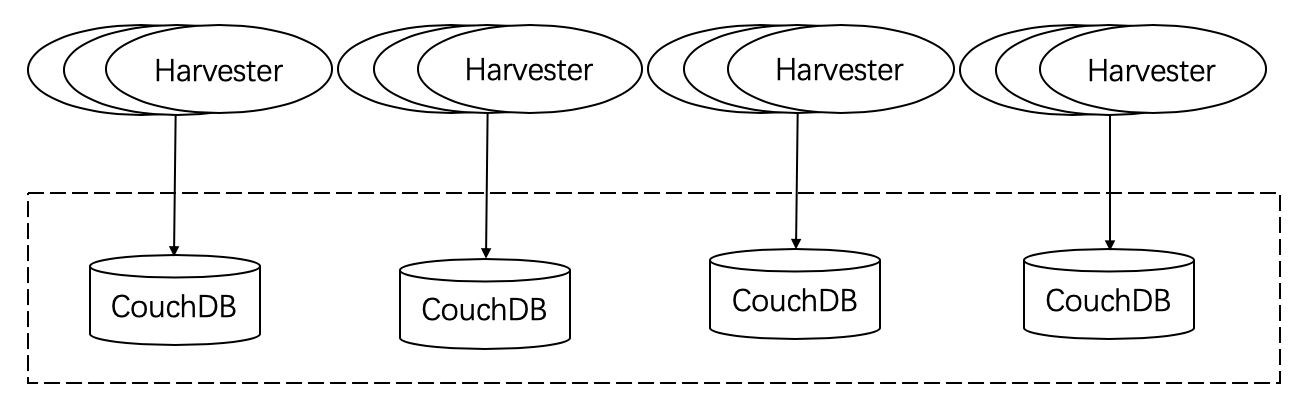
\includegraphics[width=\textwidth]{img/harvester_architecture.jpg}
\caption{the Architecture for Twitter Harvester}
\label{fig:harvester_architecture}
\end{figure}

\subsubsection{Search API}
Twitter Search API is a part of REST APIs. It is retrospective and will capture tweets in the last 7 days. We can query and gather tweets for a specific location, a specific time period or with certain interesting keywords through Search API. In this part, we specify location by the city bounding box, which is represented by the range of longitude and latitude. As each tweet has the unique tweet ID, the duplicate tweets are easy to recognize and cannot be stored in the \textit{CouchDB}, of which the details will be explained in the data processing section.

There are some limitations of mining twitter content when using the Search APIs:
\begin{itemize}
    \item The first limitation is that for per-user authentication, one can only send 180 requests per 15 minutes with the maximum of 100 tweets for each request, resulting in a total limit of 18,000 tweets per 15 minutes. In order to improve the efficiency of harvesters, they need to maintain the upper limit allowed by the APIs.
    \item The second limitation is that it will not be able to get all the tweets that match search criteria, even if they are present in the desired time slot because not all of the tweets will be indexable or made available.
    \item The third limitation is that the Search API focuses on matching the search condition (relevance) rather than all the eligible tweets (completeness) as some users and tweets will be missing during the usage of Search API
    \cite{Standard-search}.But Streaming API is match for completeness, which will be introduced in the following subsection.
\end{itemize}
To overcome these limitations and improve the efficiency of harvesters, we come up with several solutions:
\begin{itemize}
    \item In the development phase, we get \textit{friends\_id} of users and gather tweets for each user and their friends. This method helps us capture most tweets as the request limitation per 15-min window for per user authentication is 900 and request limitation per 24-hour window is 100000 with up to a maximum of 200 tweets per distinct request. Therefore, we can obtain up to 180,000 tweets per 15 minutes, which is ten times of the common Search API. In the implementation, we gather tweets from users’ oldest tweet ID available by the method \textit{user\_timeline()} and record the earliest crawled tweet id, which can be the value of the parameter \textit{since\_id} for next harvest iteration. In this way, we can gather substantial different tweets.
    \item Besides, in order to crawl as many tweets as possible, we make full use of all consumer and token key pairs of six accounts. Instead of harvesting tweets in the whole Australia by one account and having to sleep when they hit the limit very soon, we harvest tweets in each city by one authentication account. Therefore, it takes a long time to hit the limit and more data can be gathered. This method makes the system easier to deploy and manage as well.
    \item Moreover, another strategy we tried is to replace the authentication account with another whenever it hits the limit. However, this makes the deployment very complex, confusing and did not make good use of our parallel systems. Therefore, we discard this strategy when deployment.
\end{itemize}

\subsubsection{Streaming API}
Compared to the search API, Streaming API can give developers a lower-latency access to twitter’s global stream of tweet data
\cite{streaming-data}. Also, Streaming API has a persistent HTTP connection from client side to server side so that it’s a real-time delivery and can ensure the completeness of tweets as it can gain more tweets than the search API. For example, the Search API works in a request-reply (RR) way. However, the streaming API is different in the way the server responds. The server would send a response to the client whenever a tweet is available, therefore, a continuous stream of responses will come to the client from the server and the message will appear into the stream immediately with minimal overhead. And in this part, we specify place by the city \textit{place\_id} in tweets.

Unlike Search API, Streaming API does not limit the amount of tweets harvested per time slot and it supports collecting the complete intraday tweets
\cite{streaming-data}. Therefore, for intraday tweet data, the Streaming API will theoretically capture more valid tweets than the Search API. Nonetheless, these tweet data are only the fraction of numerous eligible tweets.

\subsection{Data Processing}
In this section, the data processing steps to support the analysis scenarios will be discussed.
\subsubsection{Architecture}
Our analysis system generally follows the common pattern of data analysis: gather data -> save data -> analyze data -> present data. The architecture shows in Figure
\ref{fig:data_process_architecture}. The data processing part supported by \textit{CouchDB} then connects the Tweet harvesters, the analyzer module, and the backend together as an integrated system. Harvested tweets will be cleaned up, transformed, and saved to the database. Obtaining the data from the database by using views filtered through \textit{MapReduce}, the analyzer is able to further generate an analysis result for the given data, and save the result or update the existing result to the analysis result database. The backend fetches the result to the frontend for presenting.
\begin{figure}[htp]
\centering
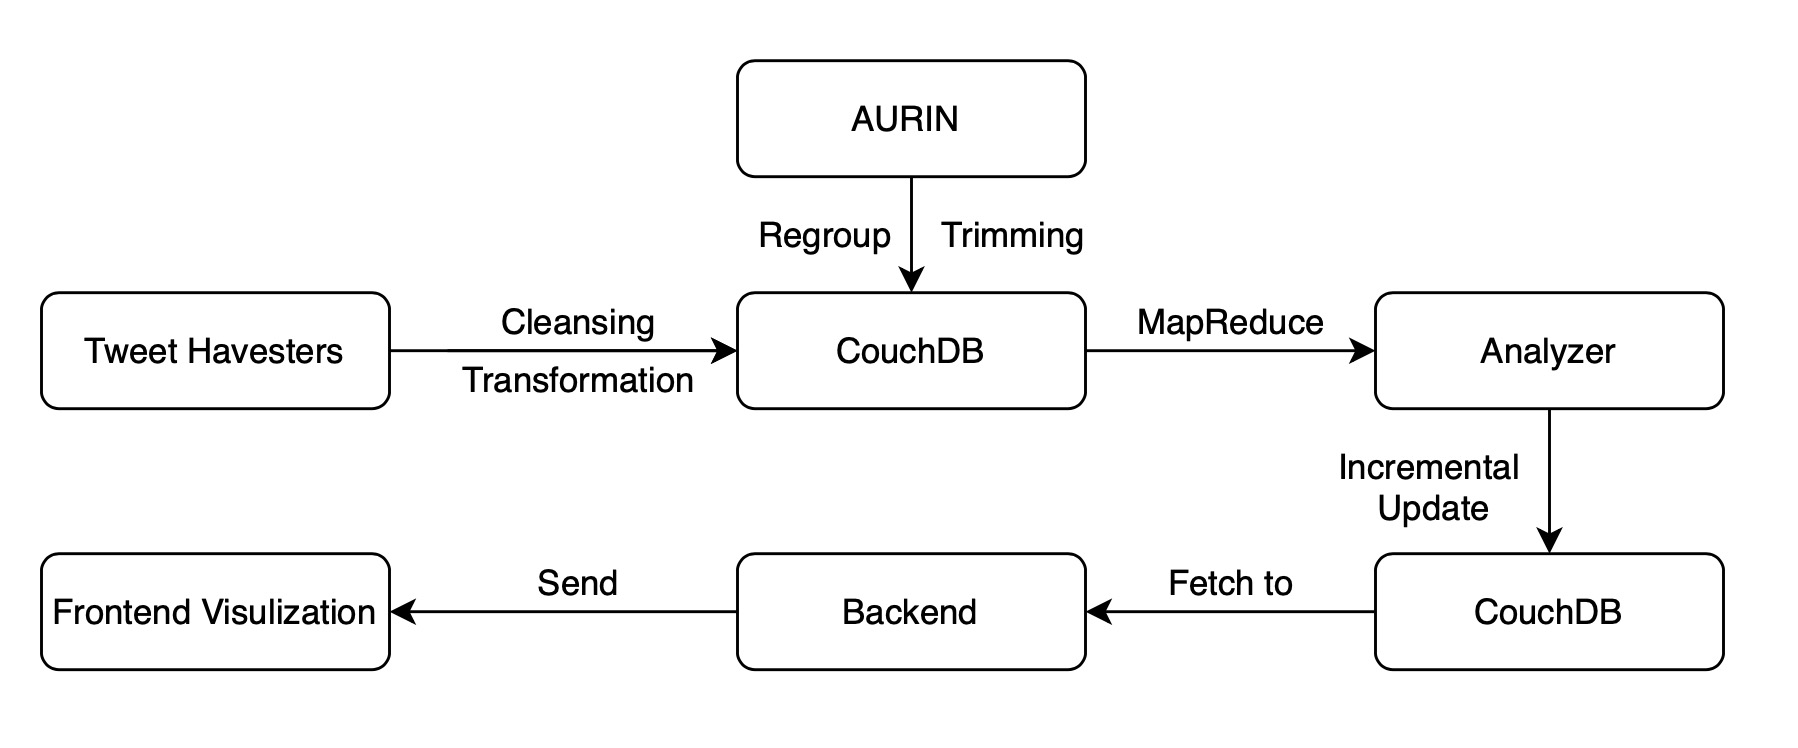
\includegraphics[width=\textwidth]{img/3_2_1_data_processing.jpg}
\caption{the Flow Chart for Data Processing}
\label{fig:fig:data_process_architecture}
\end{figure}

What’s more, to have a stable and reliable system, we have implemented an Incremental Update algorithm. During the development phase, as the data volume grows to 10 million levels, the performance and stability of the system starts dropping if the data is analyzed as a whole. But with an incremental update system, each time we will only extract the latest, not-yet-analyzed data from \textit{couchdb} based on timestamps, to the analyzer, and update the previous analyse results. In such a way, there will be no need to analyze billions of tweets every time, hence improving the performance and stability of the system. What’s more, with such architecture, more flexibility is brought up to the deployment phase, as we will only need to migrate the analysis results from the development environment but not all the tweets stored. With the help of limitations on twitter API, which allows collection of only the latest data (no more than 7 days), our analysis system will be able to avoid duplicated results and work properly.
\subsubsection{Data Cleansing and Transform}
Before saving raw data from twitter and \textit{aurin} into \textit{couchDB}, we will go through a data cleansing process to filter out unnecessary data and transform the data into aligned format, which will be easier for further processes. 

\textbf{\underline{Twitter Data}}: 

In the architecture, we will collect tweets continuously from twitter API, however, the transformation of twitter data was relatively simple, as twitter has already processed its data and all data collected from twitter are ready in a synchronized format. We will extract the twitter ID from the data as the unique key for storage in \textit{couchDB}. And since there is a tweet corpus provided to the project, which means that the data are not crawled directly from twitter, we will also check if the data has ‘\_rev’, the revision reference in \textit{couchdb}. If ‘\_rev’ exists in the data, we will simply remove it before saving to avoid update conflicts. A code demonstration is shown in the figure \ref{fig:twitterdata}.
Also, with consideration on the incremental update algorithm with our design, we will need a timestamp before inserting the twitter data into our database. Hence a field named ‘db\_timestamp’ will be inserted together with each tweet stored, as illustrated in figure \ref{fig:twitterdata}. A database named ‘tweets\_mixed’ is created to hold all twitter data crawled and extracted from tweet corpus. Then the data can go through MapReduce and be analyzed in further steps.
\begin{figure}
\centering
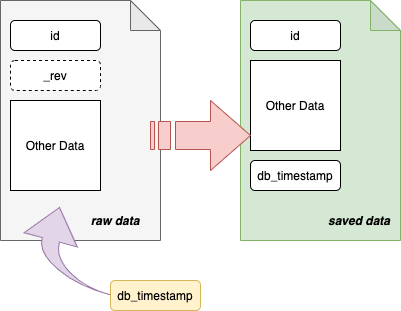
\includegraphics[width=10cm]{img/twitterdata.png}
\caption{The transformation of Twitter data}
\label{fig:twitterdata}
\end{figure}

\textbf{\underline{AURIN Data}}: 

\textit{AURIN} data is quite different from twitter data since it is not updated very often and in our project, we will not update the data from AURIN regularly. In order to make analysis based on different suburbs, we will collect multiple data sets with suburb information from AURIN. The data formats are not quite desired as they are hard for further process, hence we will re-group the information based on suburbs and extract the suburb names as keys for other information under this suburb, as shown in figure \ref{fig:aurindata} Also, some unnecessary information in the AURIN data will be removed. The data from AURIN will be saved to database ‘aurin’, and like other data, a timestamp will be inserted. But unlike tweets, we can always update a same document for AURIN, the data won’t be discarded like with tweets, but instead, the data will be updated and a latest timestamp will be inserted.
\begin{figure}[htp]
\centering
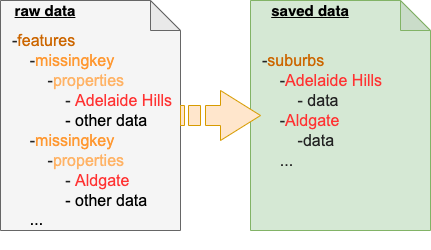
\includegraphics[width=10cm]{img/aurindata.png}
\caption{The transformation of AURIN data}
\label{fig:aurindata}
\end{figure}

\textbf{\underline{Error Handling}}: 

There are several problems met during the ETL process in both development and deployment phase and they will be addressed here.
\begin{itemize}
    \item \textbf{Duplicate tweets}: The major problem we would need to address will be the duplication of data from twitter harvesters. Both in development and deployment, there are multiple duplicate tweets collected. To address the problem, Tweet ID is used as an unique identifier (like surrogate key in relational database) to distinguish among these data. If the crawled tweet ID is already in our database, we will get an update \textbf{Resource Confict} from \textit{couchDB}, which means the data is duplicated and the data processor will ignore this tweet. Also, such an algorithm also guarantees that the incremental update of our architecture works correctly: all processed tweet IDs will not be handled twice as their timestamp won’t be changed if they have been saved to our database. We implement this based on the assumption that twitter won’t update its data if the tweet is already saved into their system, so we won’t have any data loss.

    \item \textbf{Timestamps update}: During the development phase, we firstly do not have a timestamp of our database system in the beginning. All the tweets collected will be processed in one time with Map Reduce. However, with the increment of data volume, the performance starts dropping quickly and we came up the idea of incremental analysis, which requires a timestamp of our own system. \textit{CouchDB} update functions in figure \ref{fig:insertts} are utilized in order to update tweets that are already saved in the database without a timestamp. With execution of the update function ‘insert\_ts’, all existing tweets in our database will be inserted with a timestamp.
\begin{figure}
\centering
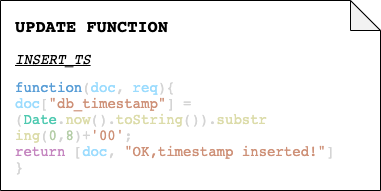
\includegraphics[width=8cm]{img/insert_ts.png}
\caption{Update function for inserting timestamp}
\label{fig:insertts}
\end{figure}
\end{itemize}

\subsubsection{Data Manipulation using \textit{CouchDB} functions}
After the twitter data is saved into the database, we will need to do some research on the data and also extract the data. Here we will utilize different \textit{Couchdb} built-in functions to study the data and extract the data.

To study the data at an early stage, we mainly relied on the text search function \footnote{https://docs.couchdb.org/en/master/ddocs/search.html}. For example, at the very beginning, we were trying to make an analysis on most popular car brands with their most mentioned factors mentioned in tweets, and their relations to the poor and wealthy suburbs in Australia. We have used text search functions in \textit{Couchdb} to search for different brands. However, as twitter limited us to collect only data for the past 7 days, it turns out there are very few tweets mentioning automobiles. So we have abandoned the scenario, but \textit{CouchDB} built-in functions have indeed made the study of data easier.

To extract the data in later stages, we have turned into MapReduce views \footnote{https://docs.couchdb.org/en/stable/ddocs/views/intro.html} in \textit{CouchDB}. Although with the previous data processing steps, we have limited the tweet data we collected in some way, however, there are still many redundant data that is not fit for our scenarios. We kept these data in the database with consideration on further usage, but in the current stage, we would not feed such data into the analysis phase. But it will be very much complicated and resources consuming if we are going to filter out such data one by one. Also, as introduced in section 3.2.1, our analyzer system uses an incremental update method. So for each epoch, only the latest collected tweets that have not been analyzed will be extracted and passed to the analysis module. MapReduce function in \textit{couchDB} will be used to make life easier. Besides, the views created with MapReduce will also assist in the analysis process.

There will be two views created in the system to assist in the analysis process, kes of whome demonstrated in figure \ref{mapreduce}. The fist one is named \textit{‘by\_city’}, which is used to extract data by city name and count the number of tweets within the specified city. This view will be used mostly to inspect data and in calculating ratios with the total number of tweets in a city.
\begin{figure}[hbp]
\centering
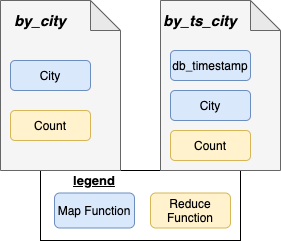
\includegraphics{img/mapreduce.png}
\caption{Function structure of MapReduce views}
\label{fig:mapreduce}
\end{figure}

The other one is named \textit{‘by\_city\_ts’}, which can extract tweets of a certain city by the timestamp that it was inserted into our system. This is the main view we will use in our incremental update analyzer module, where we will get only the latest data that is not analyzed before, determined by the timestamp. Also a count reduce function is implemented with this view to get statistics on the data processed in each ‘increment’.

\subsection{Analyzer Module}
The analyzer module supports six scenarios which include three city-level scenarios and three suburb-level scenarios, and the details of each scenario will be introduced in the ‘Analytic Scenarios’ part of this report.
\subsubsection{Analysis Result Structure}
The analysis results for the scenarios are saved in the database for the frontend further presenting. The structure of the result contains three layers and can be load from result.structure.cfg configuration file. The first layer contains the city name, city tweet counts, and keys for the second layer values. The second layer contains the city-level analysis and the suburb keys. The third layer contains suburb-level analysis.
\subsubsection{Static Result Manager}
The job of the static result manager is handling the data obtained from AURIN. Theoretically, this part of the analysis result will not be changed after the first time it is loaded to the database. The AURIN data is stored in the database according to different scenarios and different cities. The manager fetches data from the database, picks the valuable data chucks and fills them into the result structure. The manager is also able to decide which parts of data should be load.
\subsubsection{Dynamic Result Manager (Tweet Analyzer)}
The tweet analyzer has two modes, one is generating analysis results from the given historical tweets, and one is non-stop analyzing newcome tweets and updating the existing result. While the whole system is running on the cloud, the mode used is the second one. 

As more tweet data coming into the database, it is necessary to make sure that the analysis result is up-to-date. Therefore, the analysis result in the database should be dynamic. The way to achieve that is running the tweet analyzer every period t (which now is set to be 1000 seconds), and each time the analyzer will get the newcome tweets from the past period t and analyze them. After analyzing, the tweet analyzer will update the existing analysis result in the database, and sleep until the next wake up. The tweet analyzer also has a logger that logs whether the analyzer is running or sleeping, the timestamps of the tweets have been analyzed and any potential errors. The group member in charge of the server will, therefore, be easily monitoring the status of the analyzer.

There are three main functionalities designed for city-level scenarios. The first one is identifying whether the tweet mentions COVID\-19, and if it does, then get the number of followers that the tweet poster has. The analyzer will check if the keywords like ‘COVID’ or ‘coronavirus’ appear in the tweet text, hashtags, or links. Follower counting is done by using Twitter API \textit{get\_user().followers\_count}. The second one is identifying whether the tweeting time is at night and whether the location label is enabled. Transforming UTC time in tweet JSON to AEST and finding the coordinates value of key ‘geo’ are the main steps. Lastly, counting the number of unique users and therefore calculating the tweeting density, which is the number of tweets per user.

In terms of suburb-level scenarios, the analyzer will first try to match the tweet to a specific suburb based on the coordinates of the tweet and the boundaries of the city suburbs. It is done by using Polygon and Point classes in package shapely.geometry. The analyzer uses package vadarSentiment to identify the sentiment of a tweet, and the sentiment can be positive, negative, or neutral. The analyzer uses package profanity for searching profanity in the tweet’s text. The tweeting language is simply identified from the value of key ‘lang’ in tweet JSON.
\subsubsection{Database Connector}
Database Connector contains two main parts, data loader and analysis result saver. The data loader helps the other parts of the analyzer module load different data according to different needs. Loading Twitter data by timestamps or by cities, loading the city map coordinates, and loading AURIN data for certain scenarios on certain suburbs are examples of what the data loader is able to do.

Analysis result saver is able to simply replace or incremental update the existing analysis result with the new result. The reason why the result saver has this design is the thinking of incremental computing. It is necessary to consider the efficiency and performance of the system since we are doing a cloud computing project like this. The analysis is on big data, although our analysis is only based on millions of tweets, it would be unrealistic to analyze all the data at the same time when the data amount grows to a certain level. 

Dynamic Updating works on the basis of MapReduce algorithm and recursive functions. After generating the analysis result for the data filtered through MapReduce, the result saver will also fetch the existing result, then check each key in each layer of the result structure, to see whether it needs to be updated or should keep it as it is. Like for numbers related to tweets, most of the time it needs to add the renewal to the existing ones. As for strings or static results, however, we may want them to remain the same.

Analysis result saver is also to reset any part of the analysis result, in case there’s a data error or something. It is also in line with the thinking of incremental computing because we don’t want to analyze all the data gain if only some parts of the result are affected by ‘dirty data’. Just reset those parts of the analysis result to let people know that they are affected and not available, and then wait for the correct version to come.

\subsection{RESTFul API server}
We provide RESTFul APIs for accessing our analysis. We use an Nginx-uWSGI-Flask framework to build our RESTFul API server. They are all running in Docker Containers and are managed by Docker Swarm. The uWSGI-Flask service is listening on port 3000, and the Reverse Proxy Nginx server would pass the request to the uWSGI-Flask service through socket protocol. The uWSGI-Flask service would only access the CouchDB on their localhost. In this way, the crash of one CouchDB would not affect other nodes. Moreover, a load-balancing Nginx server is running in Instance 1 to improve our system's availability. Details about the architecture are shown in Section \ref{sec:systemDesignAndArchitecture}.

Our RESTFul APIs provide six types of data accessing for five cities, including both city-level and suburb-level analysis of Melbourne, Sydney, Brisbane, Adelaide and Perth. 

Our Web Application also uses these RESTFul API to access the dynamic data. By separating static from dynamic traffic, the file I/O and storage consumption of our uWSGI-Flask server reduces. 

\subsection{Web Application}
The web application is composed of front-end and back-end. We use VueJs framework to implement data visualisation and Flask framework to provide APIs. The server will receive the requests from users’ browser and then return corresponding JSON data fetched from CouchDB. With unimelb VPN, you can access our web application with http://172.26.132.125/.
\subsubsection{Data Visualisation}
Our front-end web application is composed of HTML, CSS and Javascript.

Many tools and plug-ins are used to make our presentation clear and easy to understand. Google Map provided by google API is selected as our base map. We also fetch the GeoJson file of city and suburb from Aurin APIs. And the socio-economic features we got are added into those GeoJson files. As a result, it is easy and fast to present the layer of city and suburb map combined with the corresponding analysis result at the top of the base map. 
For example, the figure below shows how the Geography information is combined with analysis data.

Numbers of coordinates form the boundary of the city and its suburbs. And the shades of the color of those polygons present the distribution of varieties of socio-economic attributes. 

Moreover, we use pie charts and bar charts to represent and compare data by ChartJs.

\section{Data Visualization and Analytic Scenarios}
The Scenarios are across five main cities in Australia, Melbourne, Sydney, Brisbane, Adelaide, and Perth. There are three city-level analysis and three suburb-level analysis.
\subsection{City-level Scenarios}
\textbf{\underline{The First City Scenario}}: 

This scenario is the relationship between the number of tweets that mentioned coronavirus and the number of followers those tweets posters have. That is, are the users with more followers more likely to mention coronavirus in their tweets? There are reasons for us to come up with this scenario. Users with more followers usually have a greater sense of social responsibility than normal people, so they may care more about the virus, which is affecting everyone. Also, users would draw more attention from the public if they talk more about hot topics. Well, there’s always a reason that someone is the one with more followers. As a result, we can see that our assumption is correct. A large proportion of the tweets mentioned coronavirus is from twitter users who have more than 500 followers, but only a few of them were tweeted by users who have less than 100 followers. The situation in each city is basically the same. The analysis bar chart for this scenario is as Figure
\ref{fig:Covid-19}. 

\begin{figure}[htp]
\centering
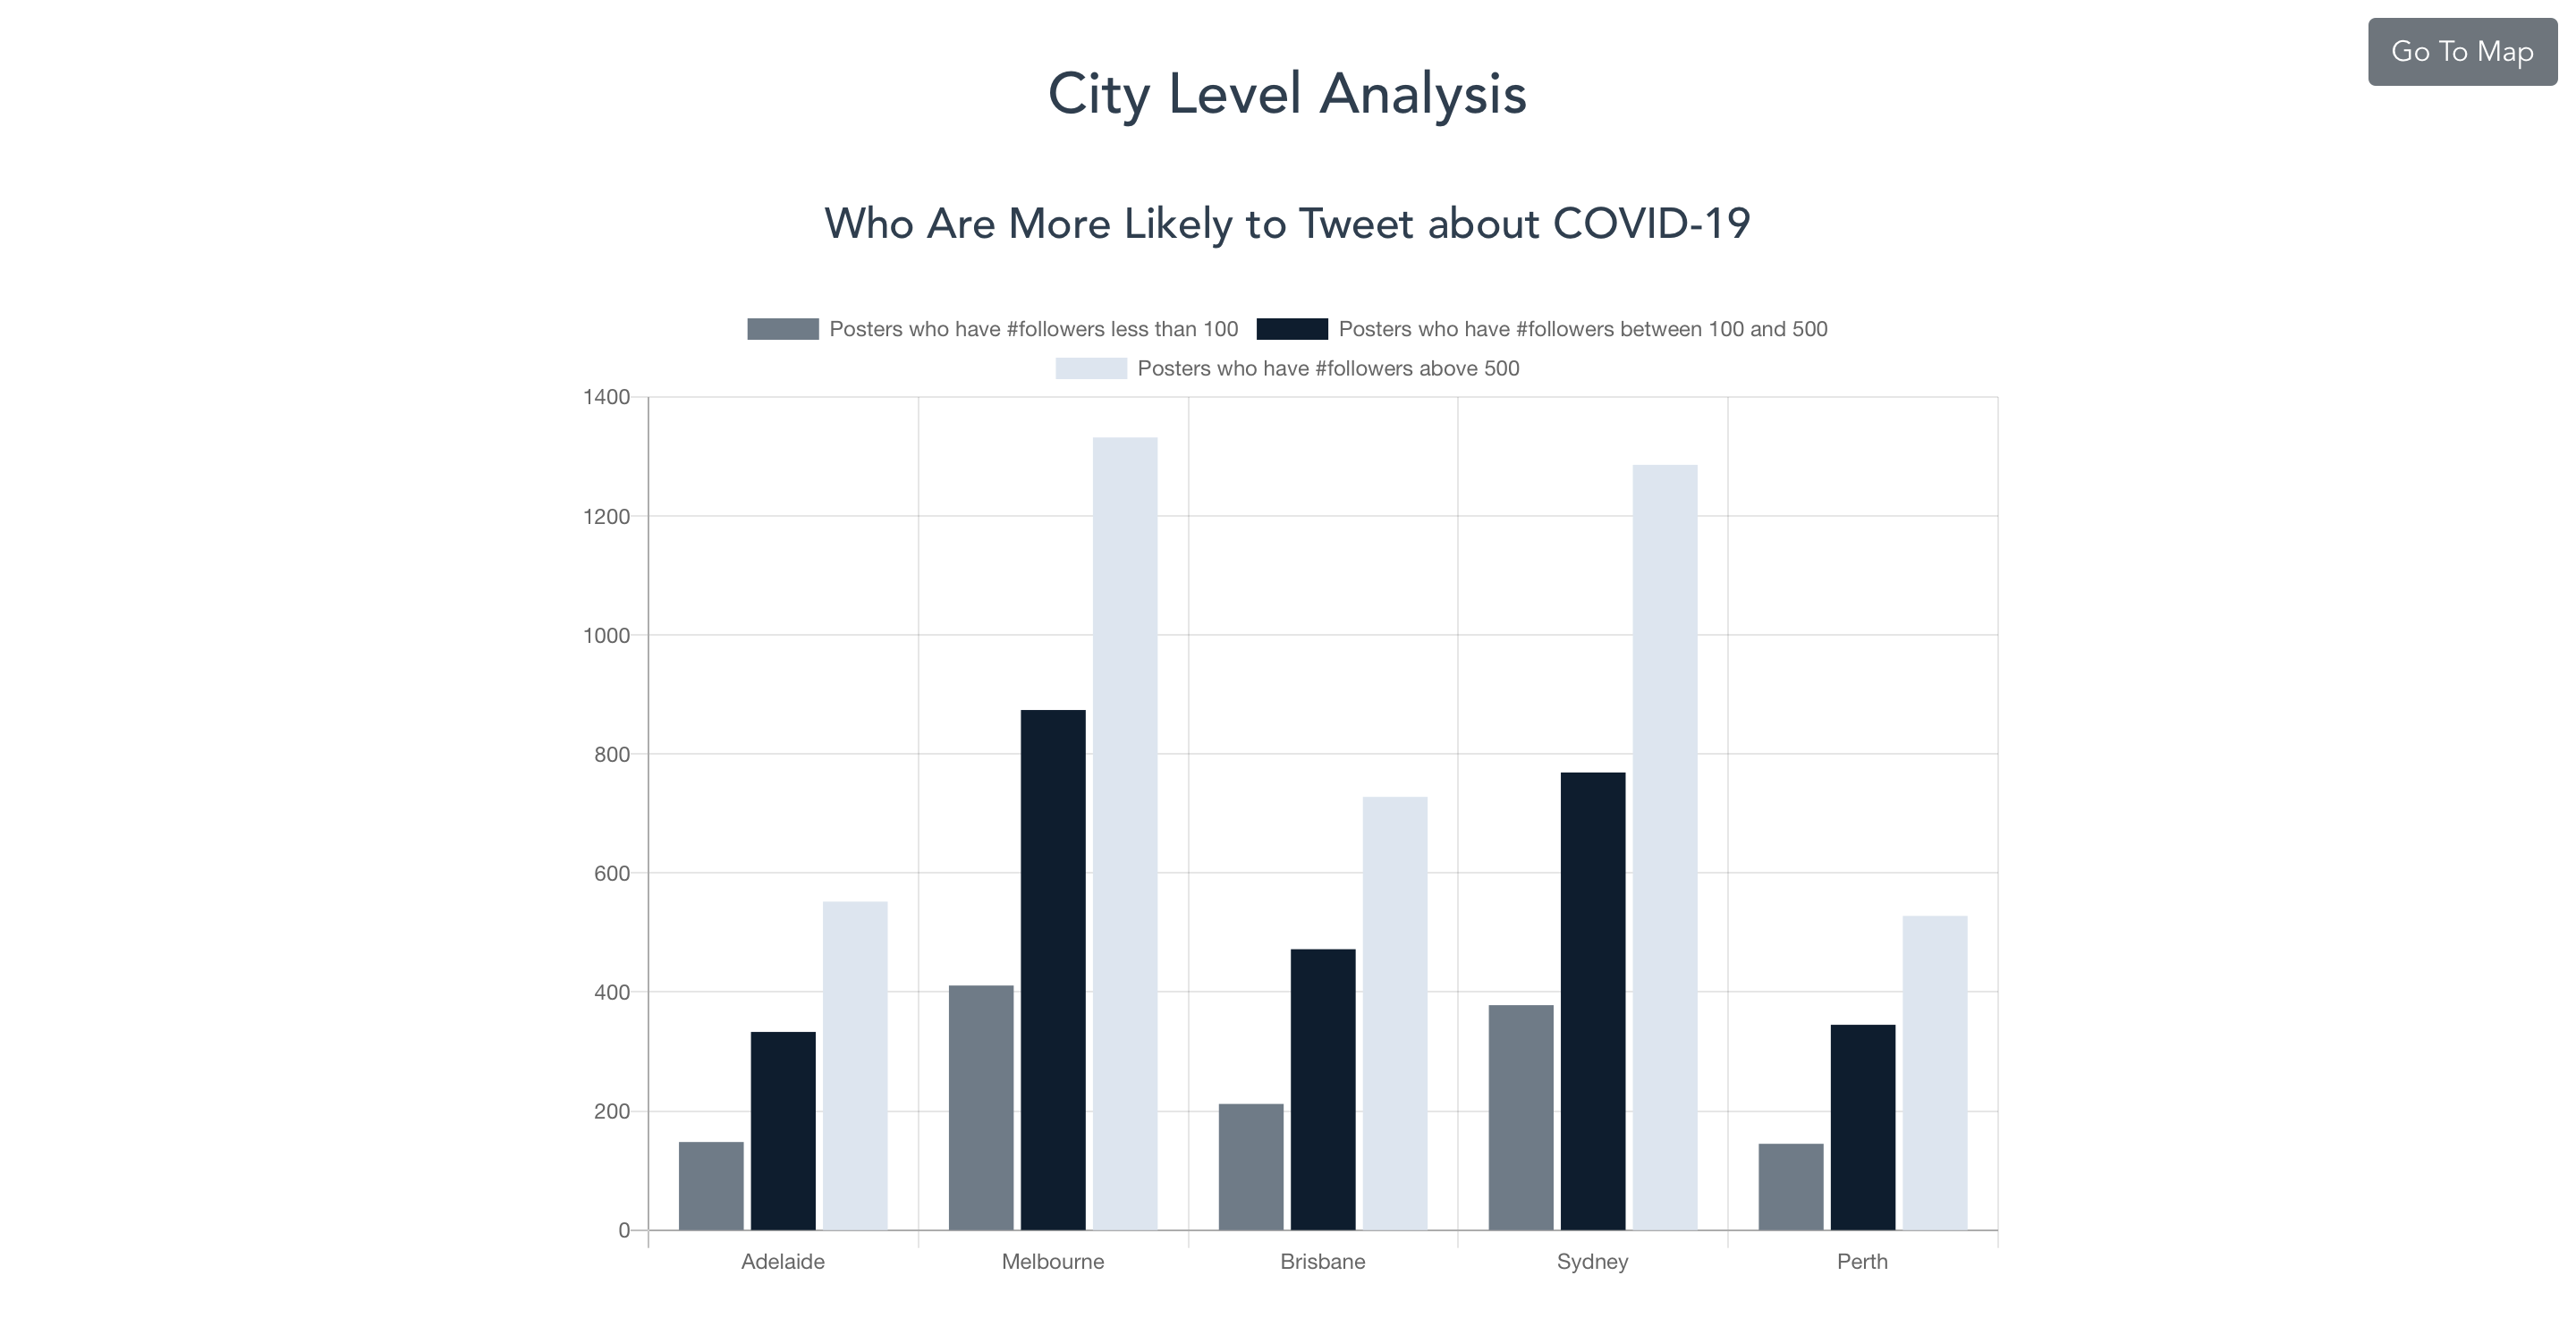
\includegraphics[width=\textwidth]{img/Covid-19.png}
\caption{Scenario 1 in city level analysis}
\label{fig:Covid-19}
\end{figure}

\textbf{\underline{the Second City Scenario}}: 

This scenario is the young people's preferences when tweeting. We would like to see whether a city has more “night tweets” and “located tweets” if the city has a larger proportion of young people. By young people, I mean people aged between 15 to 35. And night tweets are the ones that were tweeted between 11 pm to 4 am. We made a guess that young people are more likely to stay up late, and young people would love to share where they are when they tweet, to show some nice food or some fancy activities, or stuff like that, so they have their location label turned on. But the result shows that there no such relationships. It might be explained by the fact that we are in a very special period, so people don’t want to share their locations because they have nowhere to go. And Twitter might not be the night social media choice for young people. Because we also have Instagram and Facebook etc. From the plot
\ref{fig:Young_people_tweeting_preference}, we can see that Adelaide is the city with the biggest proportions of ‘located tweets’ and Perth is the city has larger ‘night tweets’ contribution.
\begin{figure}[htp]
\centering
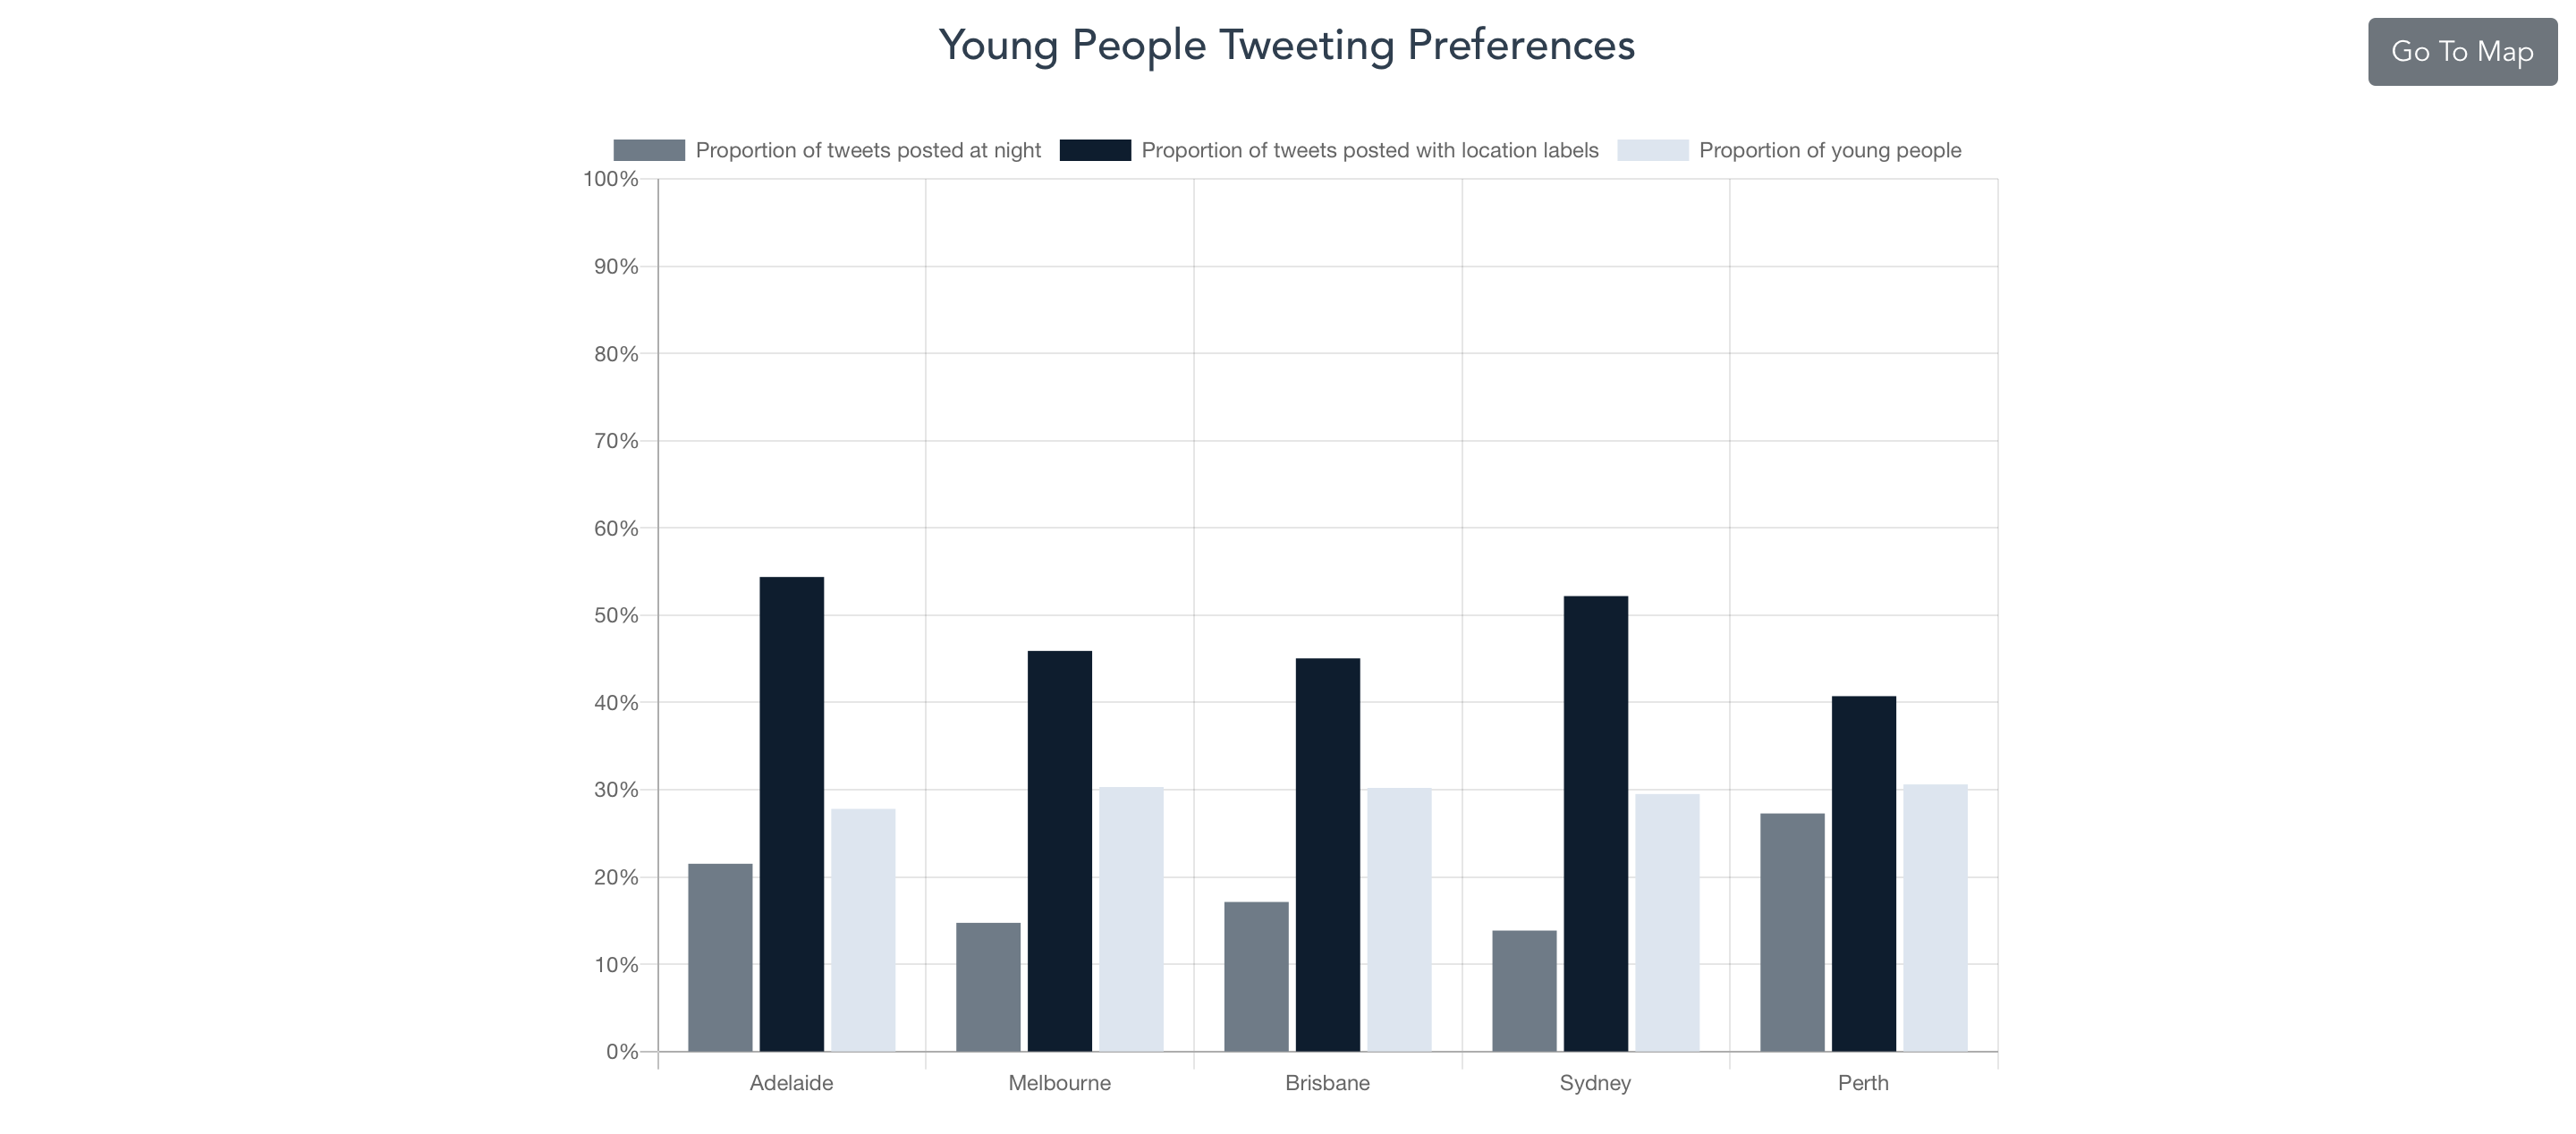
\includegraphics[width=\textwidth]{img/Young_people_tweeting_preference.png}
\caption{Scenario 2 in city level analysis}
\label{fig:Young_people_tweeting_preference}
\end{figure} 

\textbf{\underline{the Third City Scenario}}: 

This scenario is tweeting frequency versus the proportion of people who speak English as their mother tongue. I believe that most people in Australian cities do speak English at some level, but it looks like there are still many people who don’t use Twitter. I know many people whose English is good enough to tweet frequently, and do have the Twitter app on their phones, but they are not used to tweet. Therefore, we made a guess that there’s a preferred social media for each culture, and Twitter may not always be the one for cultures other than English culture. However, the result shows that cities with a lower proportion of native speakers have a relatively high tweeting density instead. For example, Melbourne has only 62\% of people whose mother tongues are English, but there are about 28 tweets per user in Melbourne. The reason might be that the more multicultural the city is, the more interesting things to tweet. Collisions between cultures always bring interesting stories. The plot 
\ref{fig:Tweeting_and_English} demonstrates this scenario.
\begin{figure}[htp]
\centering
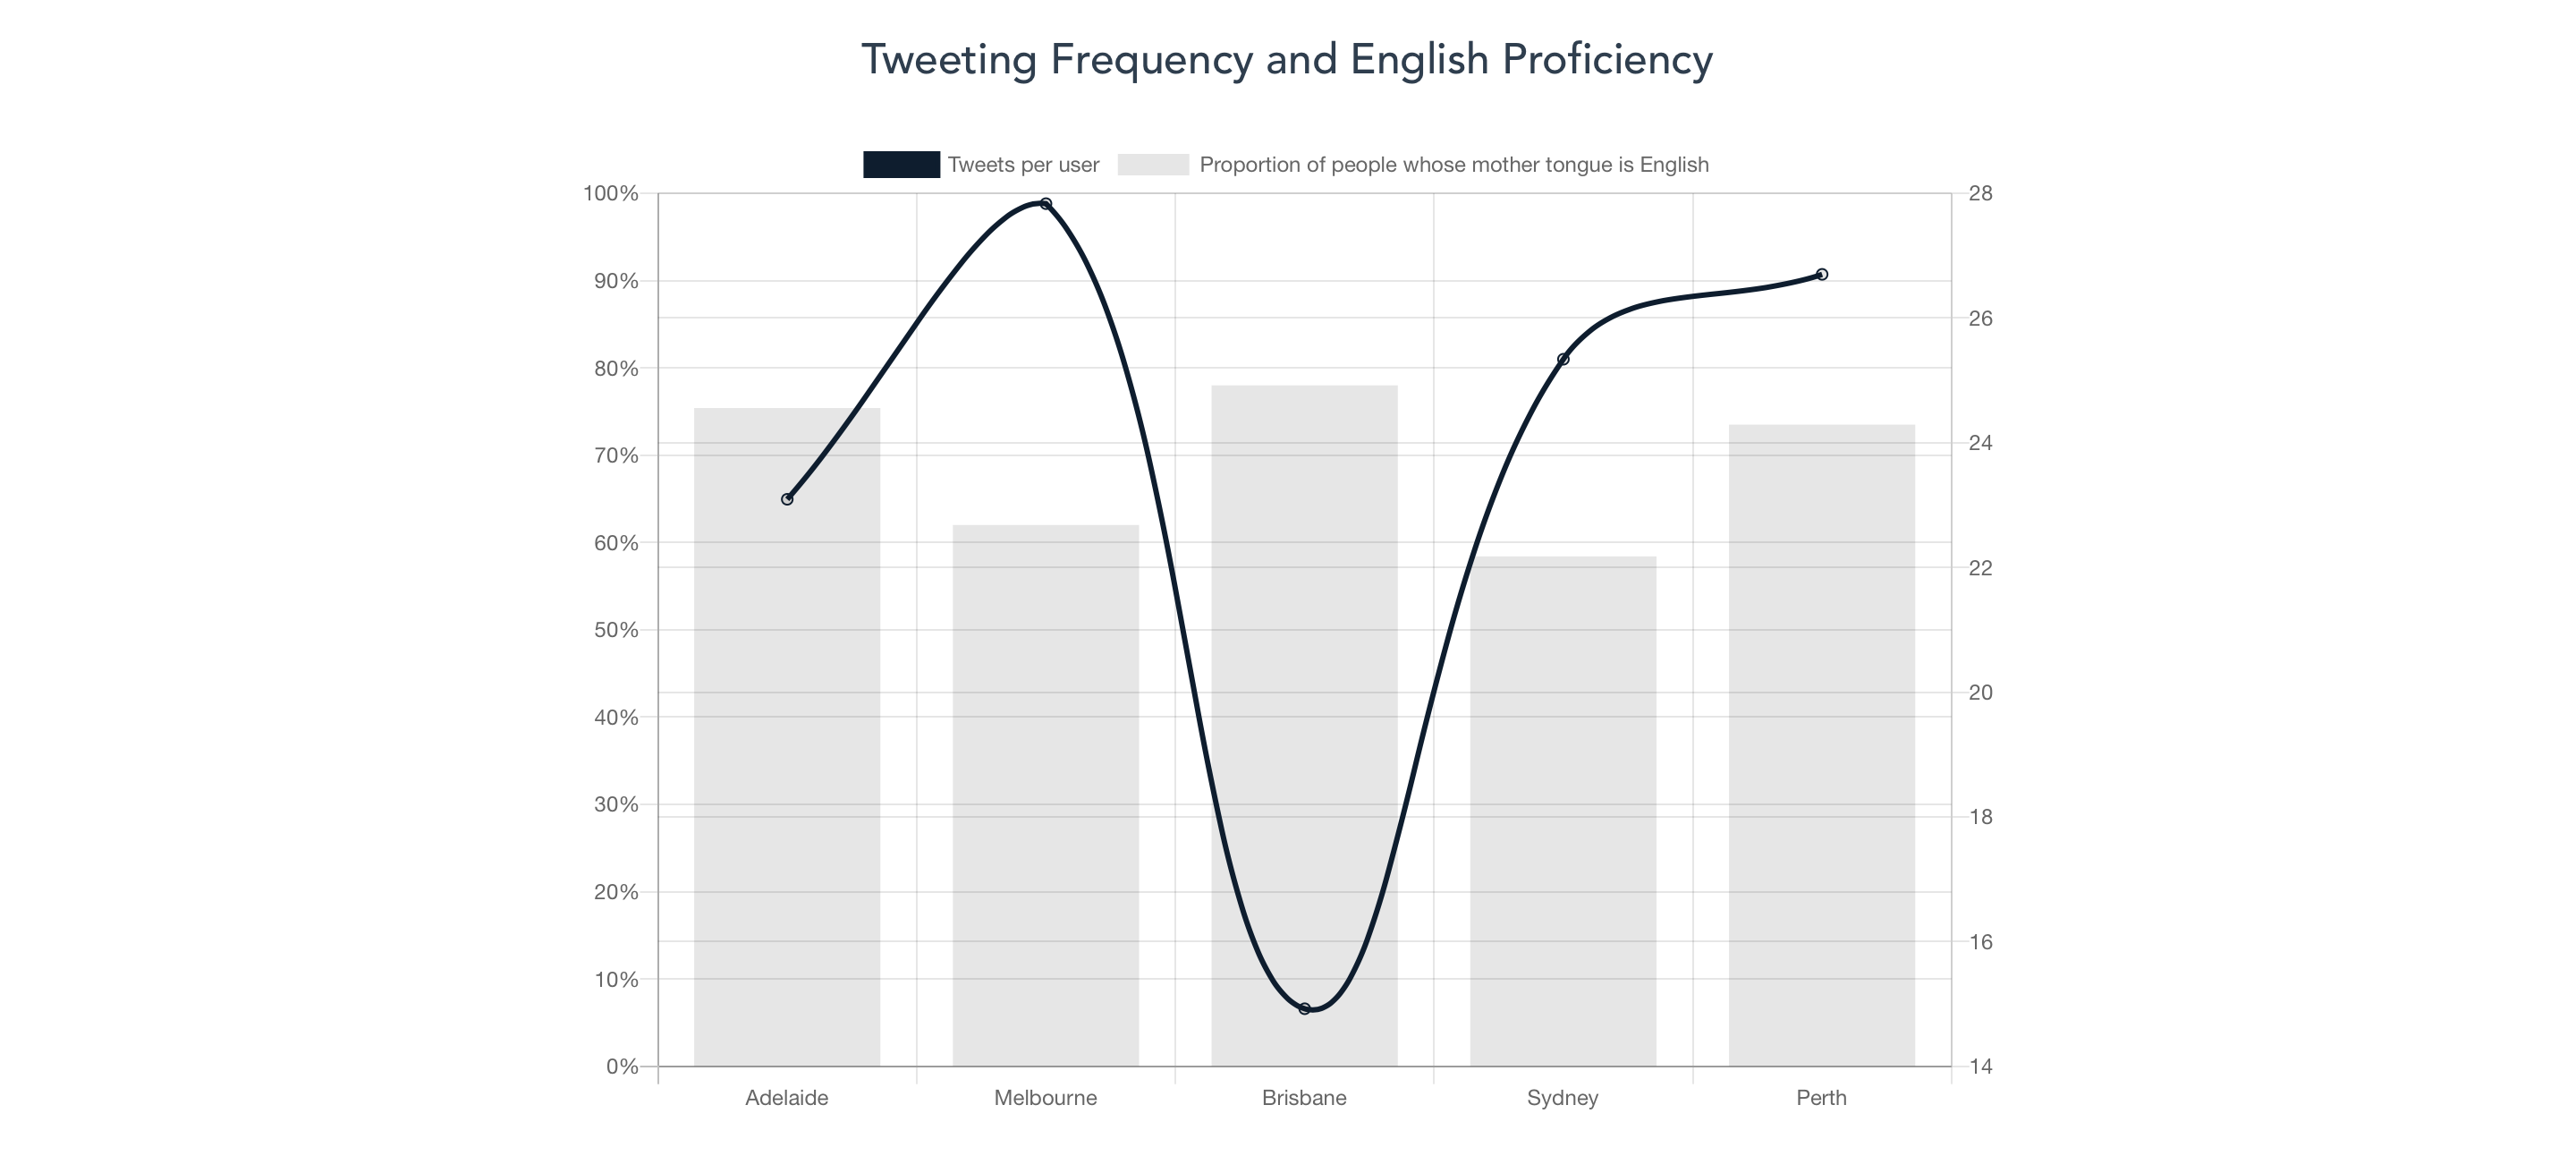
\includegraphics[width=\textwidth]{img/Tweeting_and_English.png}
\caption{scenario 3 in city level analysis}
\label{fig:Tweeting_and_English}
\end{figure} 

\subsection{Suburb-level Scenarios}
Within each city, we have gone into details and made some analysis for the suburbs in that city. For this part, we add some pie charts to the map. Whenever a suburb is clicked on, some pie charts will pop up. Each pie chart shows the distribution of each level for the corresponding attributes.

\textbf{\underline{the First Suburb Scenario}}: 

This scenario attempts to find the relationship between the proportion of income level and the tweets sentiment polarity in some city. The reason why we have this scenario is that we want to see whether people have a greater income will post more positive tweets. The color on the map in Figure
\ref{fig:Melbourne_pie_chart} represents the income level for the suburbs. The darker the color is, the higher the average income the suburb has. Here, the tweets sentiments polarity is represented as the ratio of the number of positive tweets to the number of the negative tweets. Therefore, the greater the ratio is, the more positive the emotion is. 

Let’s especially mention Melbourne city. In the map, clicking on the suburb Parkville, we can see two pie charts showing the tweets sentiment distribution and the income level  distribution in Parkville respectively. Moreover, the bar chart in Figure 
\ref{fig:Melbourne_histogram} shows the horizontal comparison across suburbs in Melbourne. Each suburb has two bars, one is the proportion of high-income people and the other one is the ratio of number of positive tweets to number of negative tweets. We can see that on the whole, the suburb with a higher proportion of high income tends to be more positive, except for some small fluctuations, like the suburbs Melbourne and Carlton. It's interesting to see that the average income is not high for these two suburbs, but the proportion of positive tweets is relatively higher than other suburbs largely. The reason we think may be there are many students in Melbourne and students are generally more positive and optimistic. This relationship is also similar for other four cities.

\begin{figure}[htp]
\centering
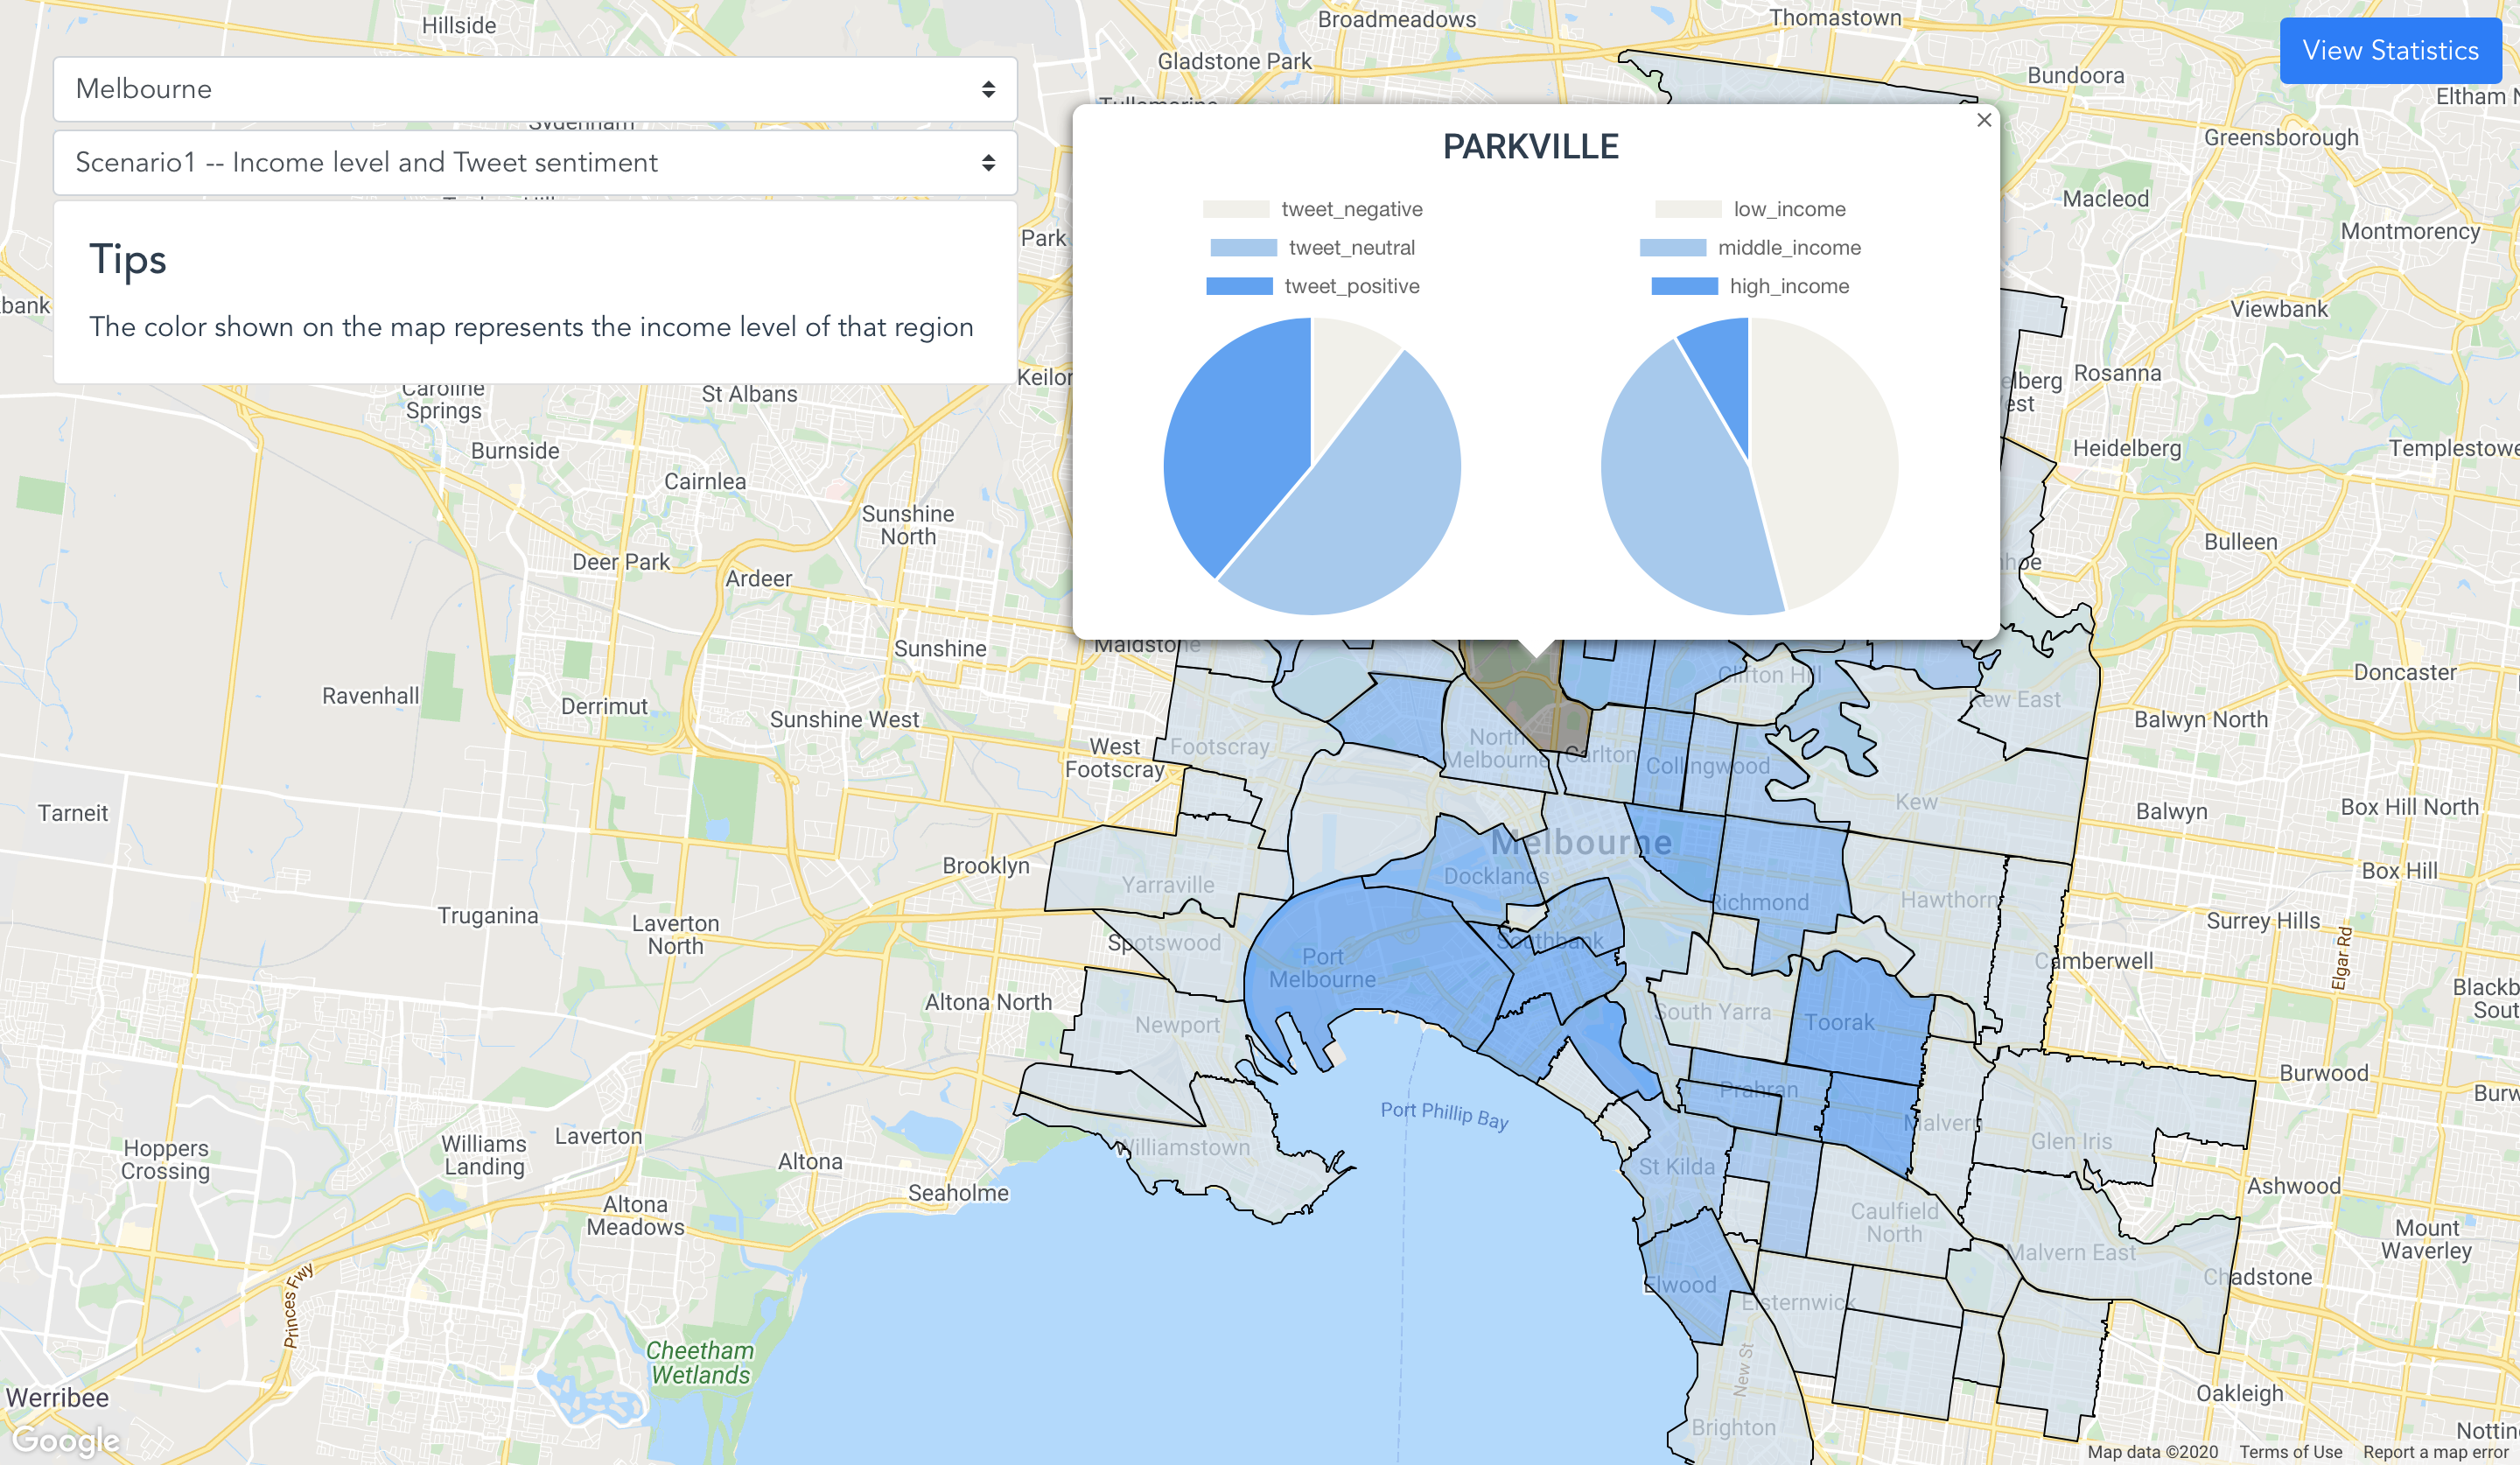
\includegraphics[width=\textwidth]{img/Melbourne_pie_chart.png}
\caption{the Pie charts in Scenario 1 for the suburb Parkille}
\label{fig:Melbourne_pie_chart}
\end{figure}

\begin{figure}[htp]
\centering
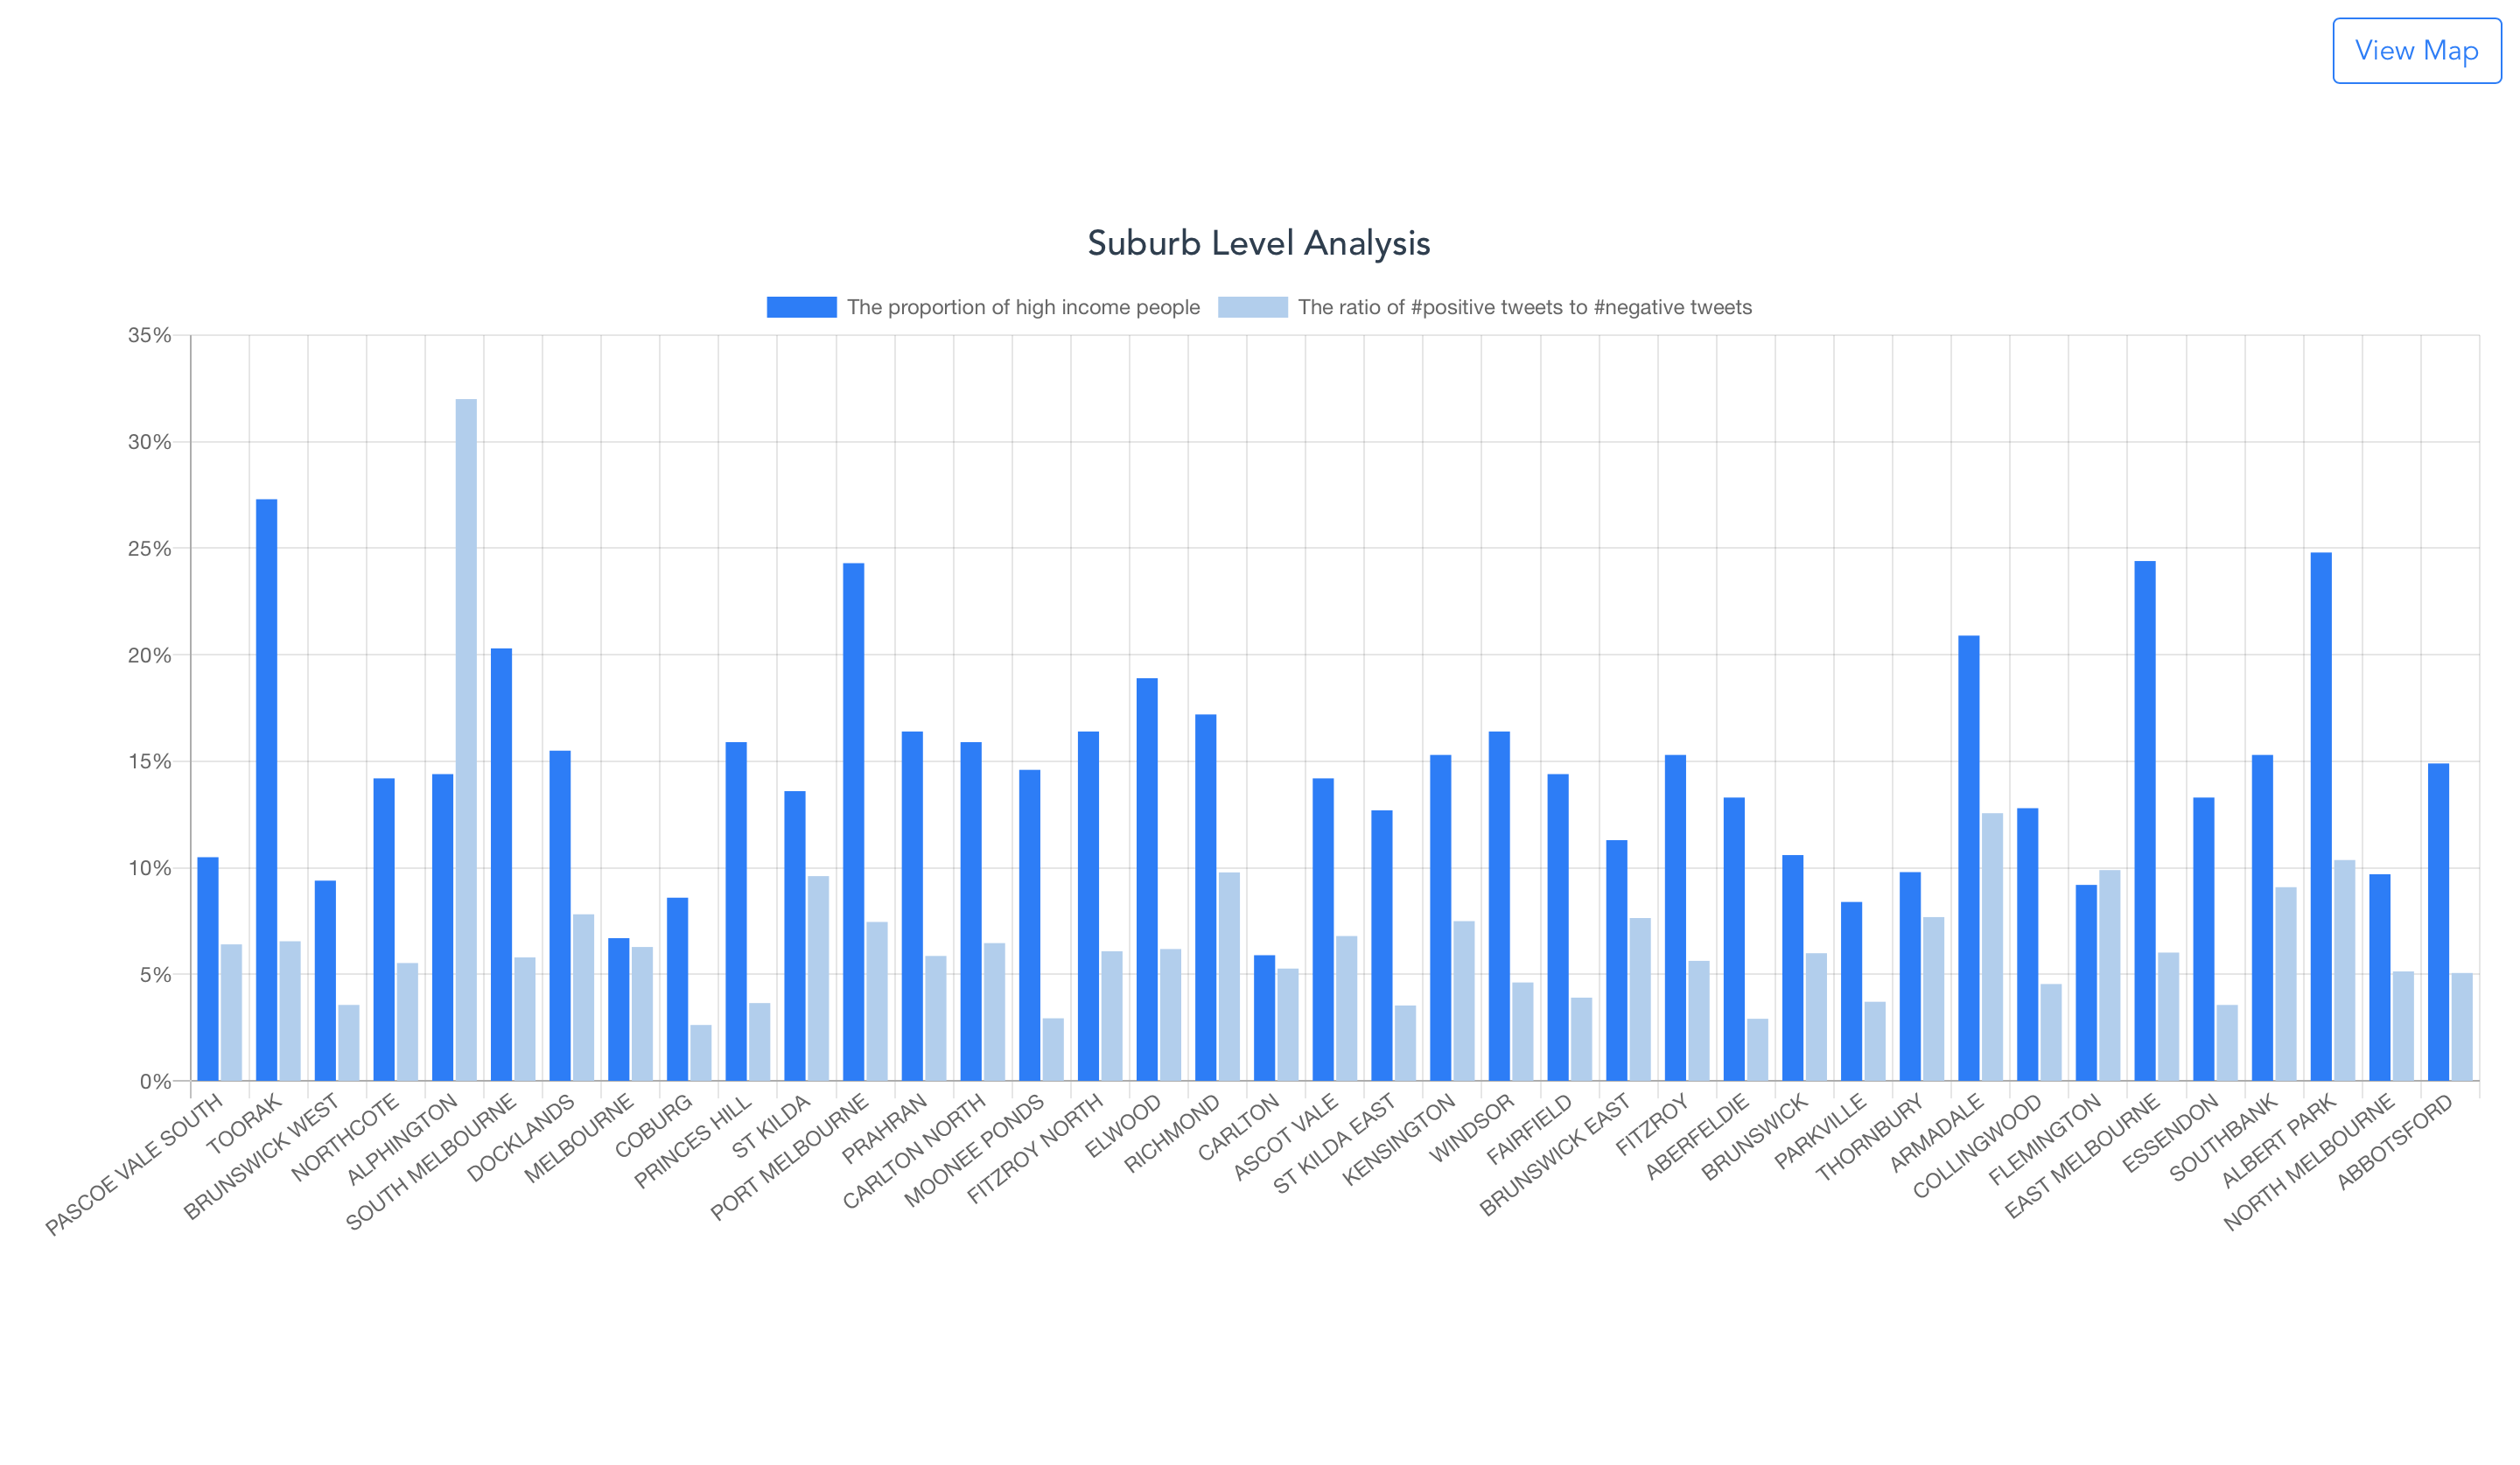
\includegraphics[width=\textwidth]{img/Melbourne_histogram.png}
\caption{the Relation between Income Level and Tweet Sentiment in Melbourne city}
\label{fig:Melbourne_histogram}
\end{figure}

\textbf{\underline{the Second Suburb Scenario}}: 

This scenario is to find if there are some relationships between the education level and the proportion of tweets containing vulgar words for each suburb in some city. Let’s take the city Sydney as an example. In the map in Figure
\ref{fig:Sydney_pie_chart}, the darker the color is, the higher vulgar tweets proportion is. Clicking the suburb Sydney, we can see there is a pie chart showing the proportion of people who have completed 12 years of education and not completed. Another pie chart shows the proportion of youth who are in study or work and who are not. These pie charts give us more details about the suburb. It’s obvious from the bar chart in Figure
\ref{fig:Sydney_histogram}, that on the whole, the suburb with a higher proportion of people with low education achievements tends to have more tweets with vulgar tweets. Similar for other cities, such as Adelaide and Perth.

\begin{figure}[htp]
\centering
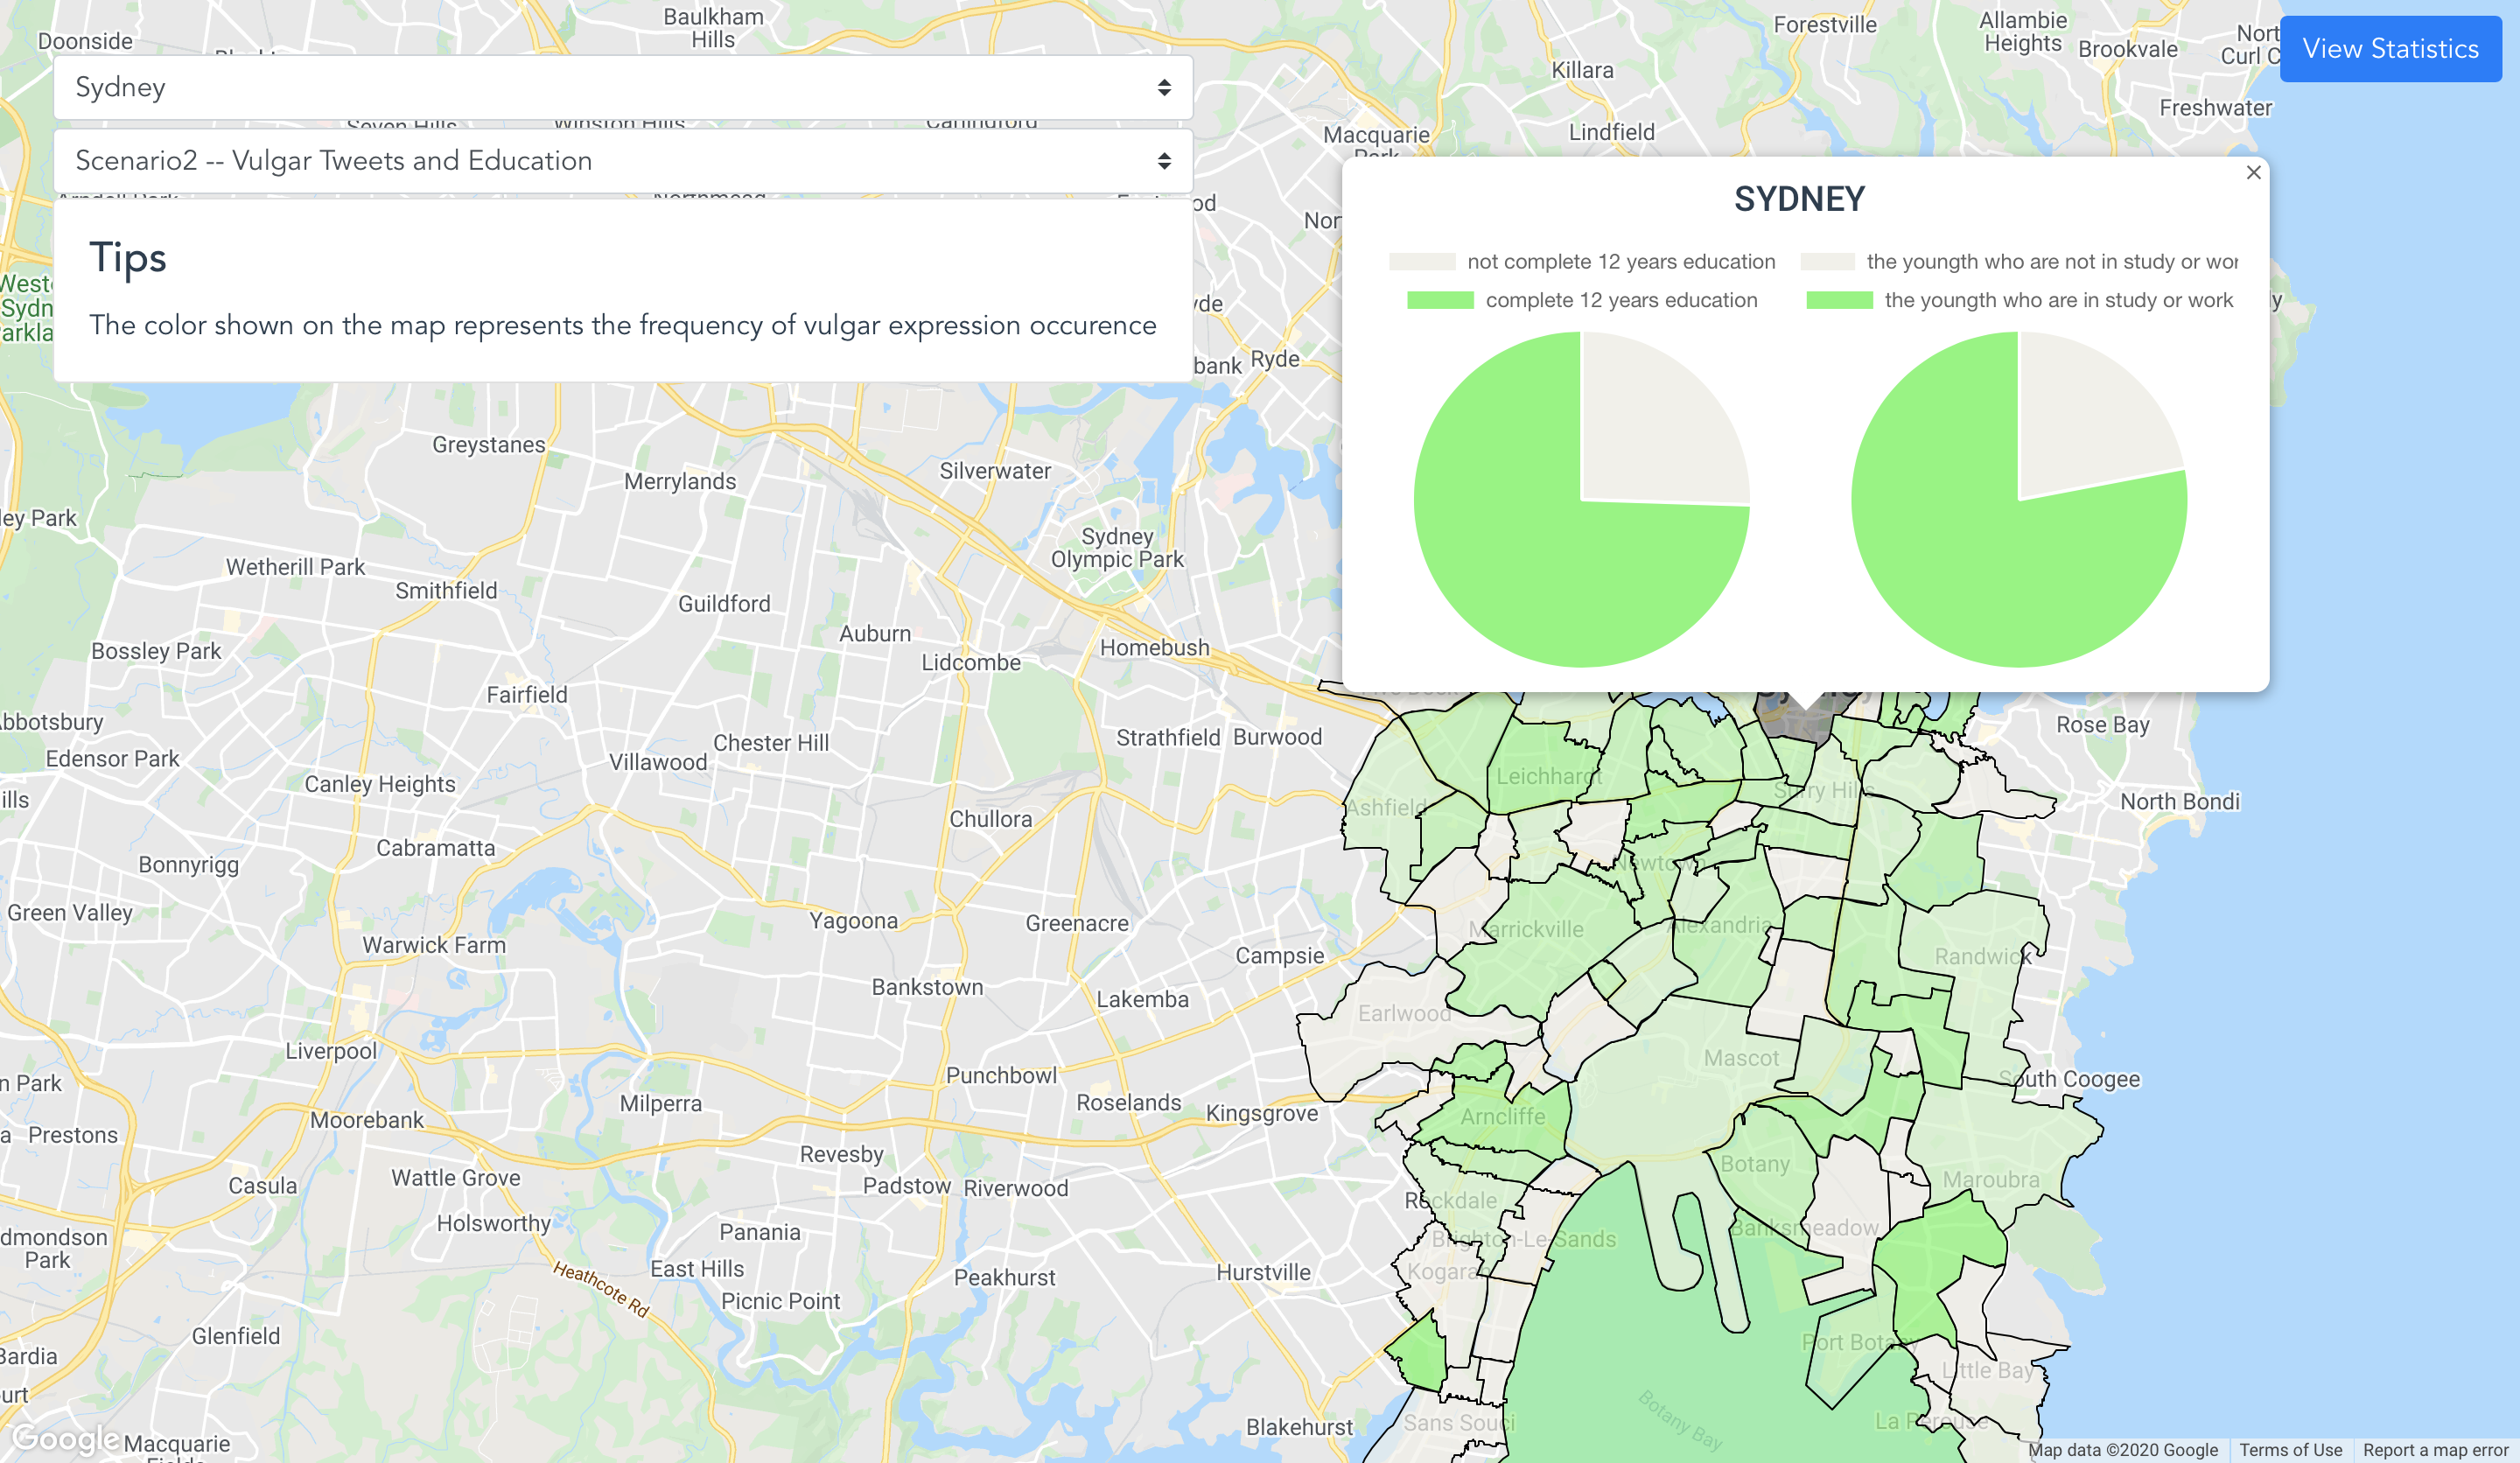
\includegraphics[width=\textwidth]{img/Sydney_pie_chart.jpg}
\caption{the Pie charts in Scenario 2 for the suburb Sydney}
\label{fig:Sydney_pie_chart}
\end{figure}

\begin{figure}[htp]
\centering
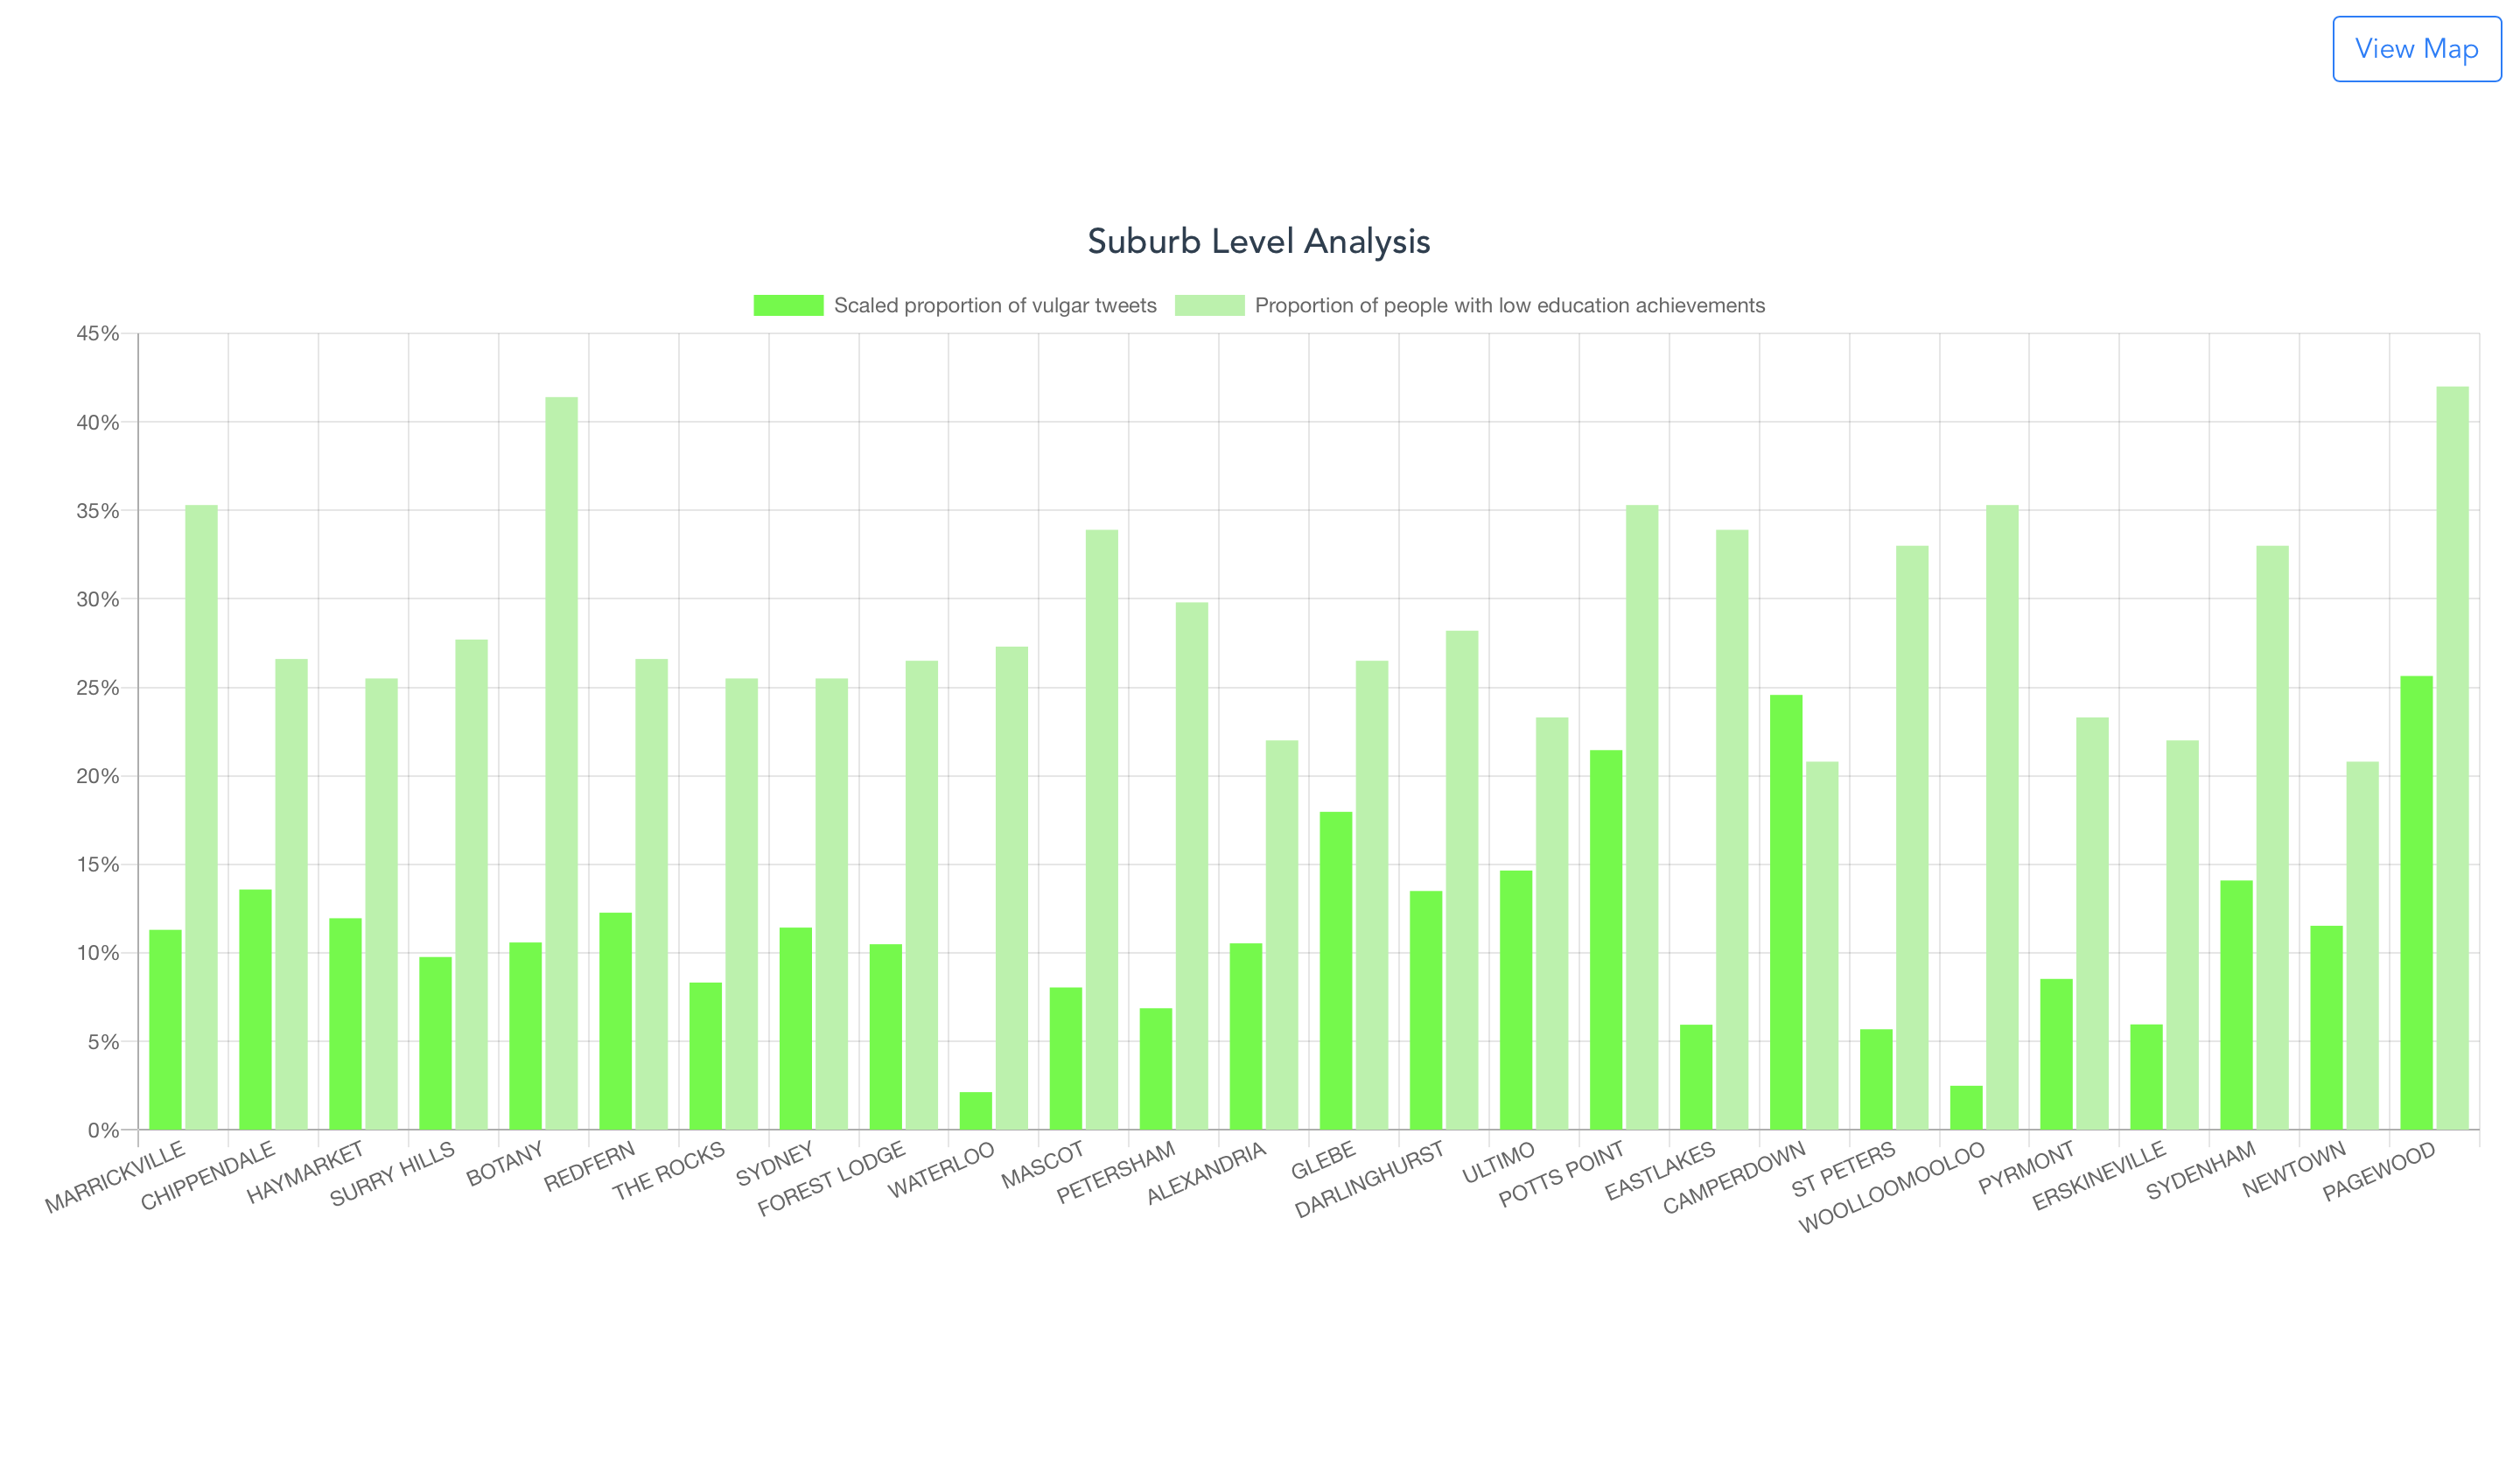
\includegraphics[width=\textwidth]{img/Sydney_histogram.jpg}
\caption{the Relation between Vulgar Tweets and Education Achievements in Sydney city}
\label{fig:Sydney_histogram}
\end{figure}

\textbf{\underline{the Third Suburb Scenario}}: 

This scenario is to detect if there is some relationship between the proportion  of non-English tweets and proportion of people who don't speak English at home in a city. For instance, in the city Perth, in the map in Figure 
\ref{fig:Perth_pie_chart}, the darker the color is, the higher the non-English tweet proportion is. Clicking the suburb Subiaco, we can see there is a pie char showing the proportion of people who speak English at home and people who do not. Another pie chart shows the proportion of people born overseas and born in Australia. From the bar chart
\ref{fig:Perth_histogram}, we can see that in general, the higher the proportion of people who don’t speak English at home, the higher the proportion of non-English tweets, except some suburbs, like Mount Claremont and Dalkeith. In Dalkeith, there is a higher proportion of people who don’t speak English at home, but a relatively lower proportion of non-English tweets, which is really weird and there are may be some reason for that. Similar for other cities, such as Sydney and Brisbane.

\begin{figure}[htp]
\centering
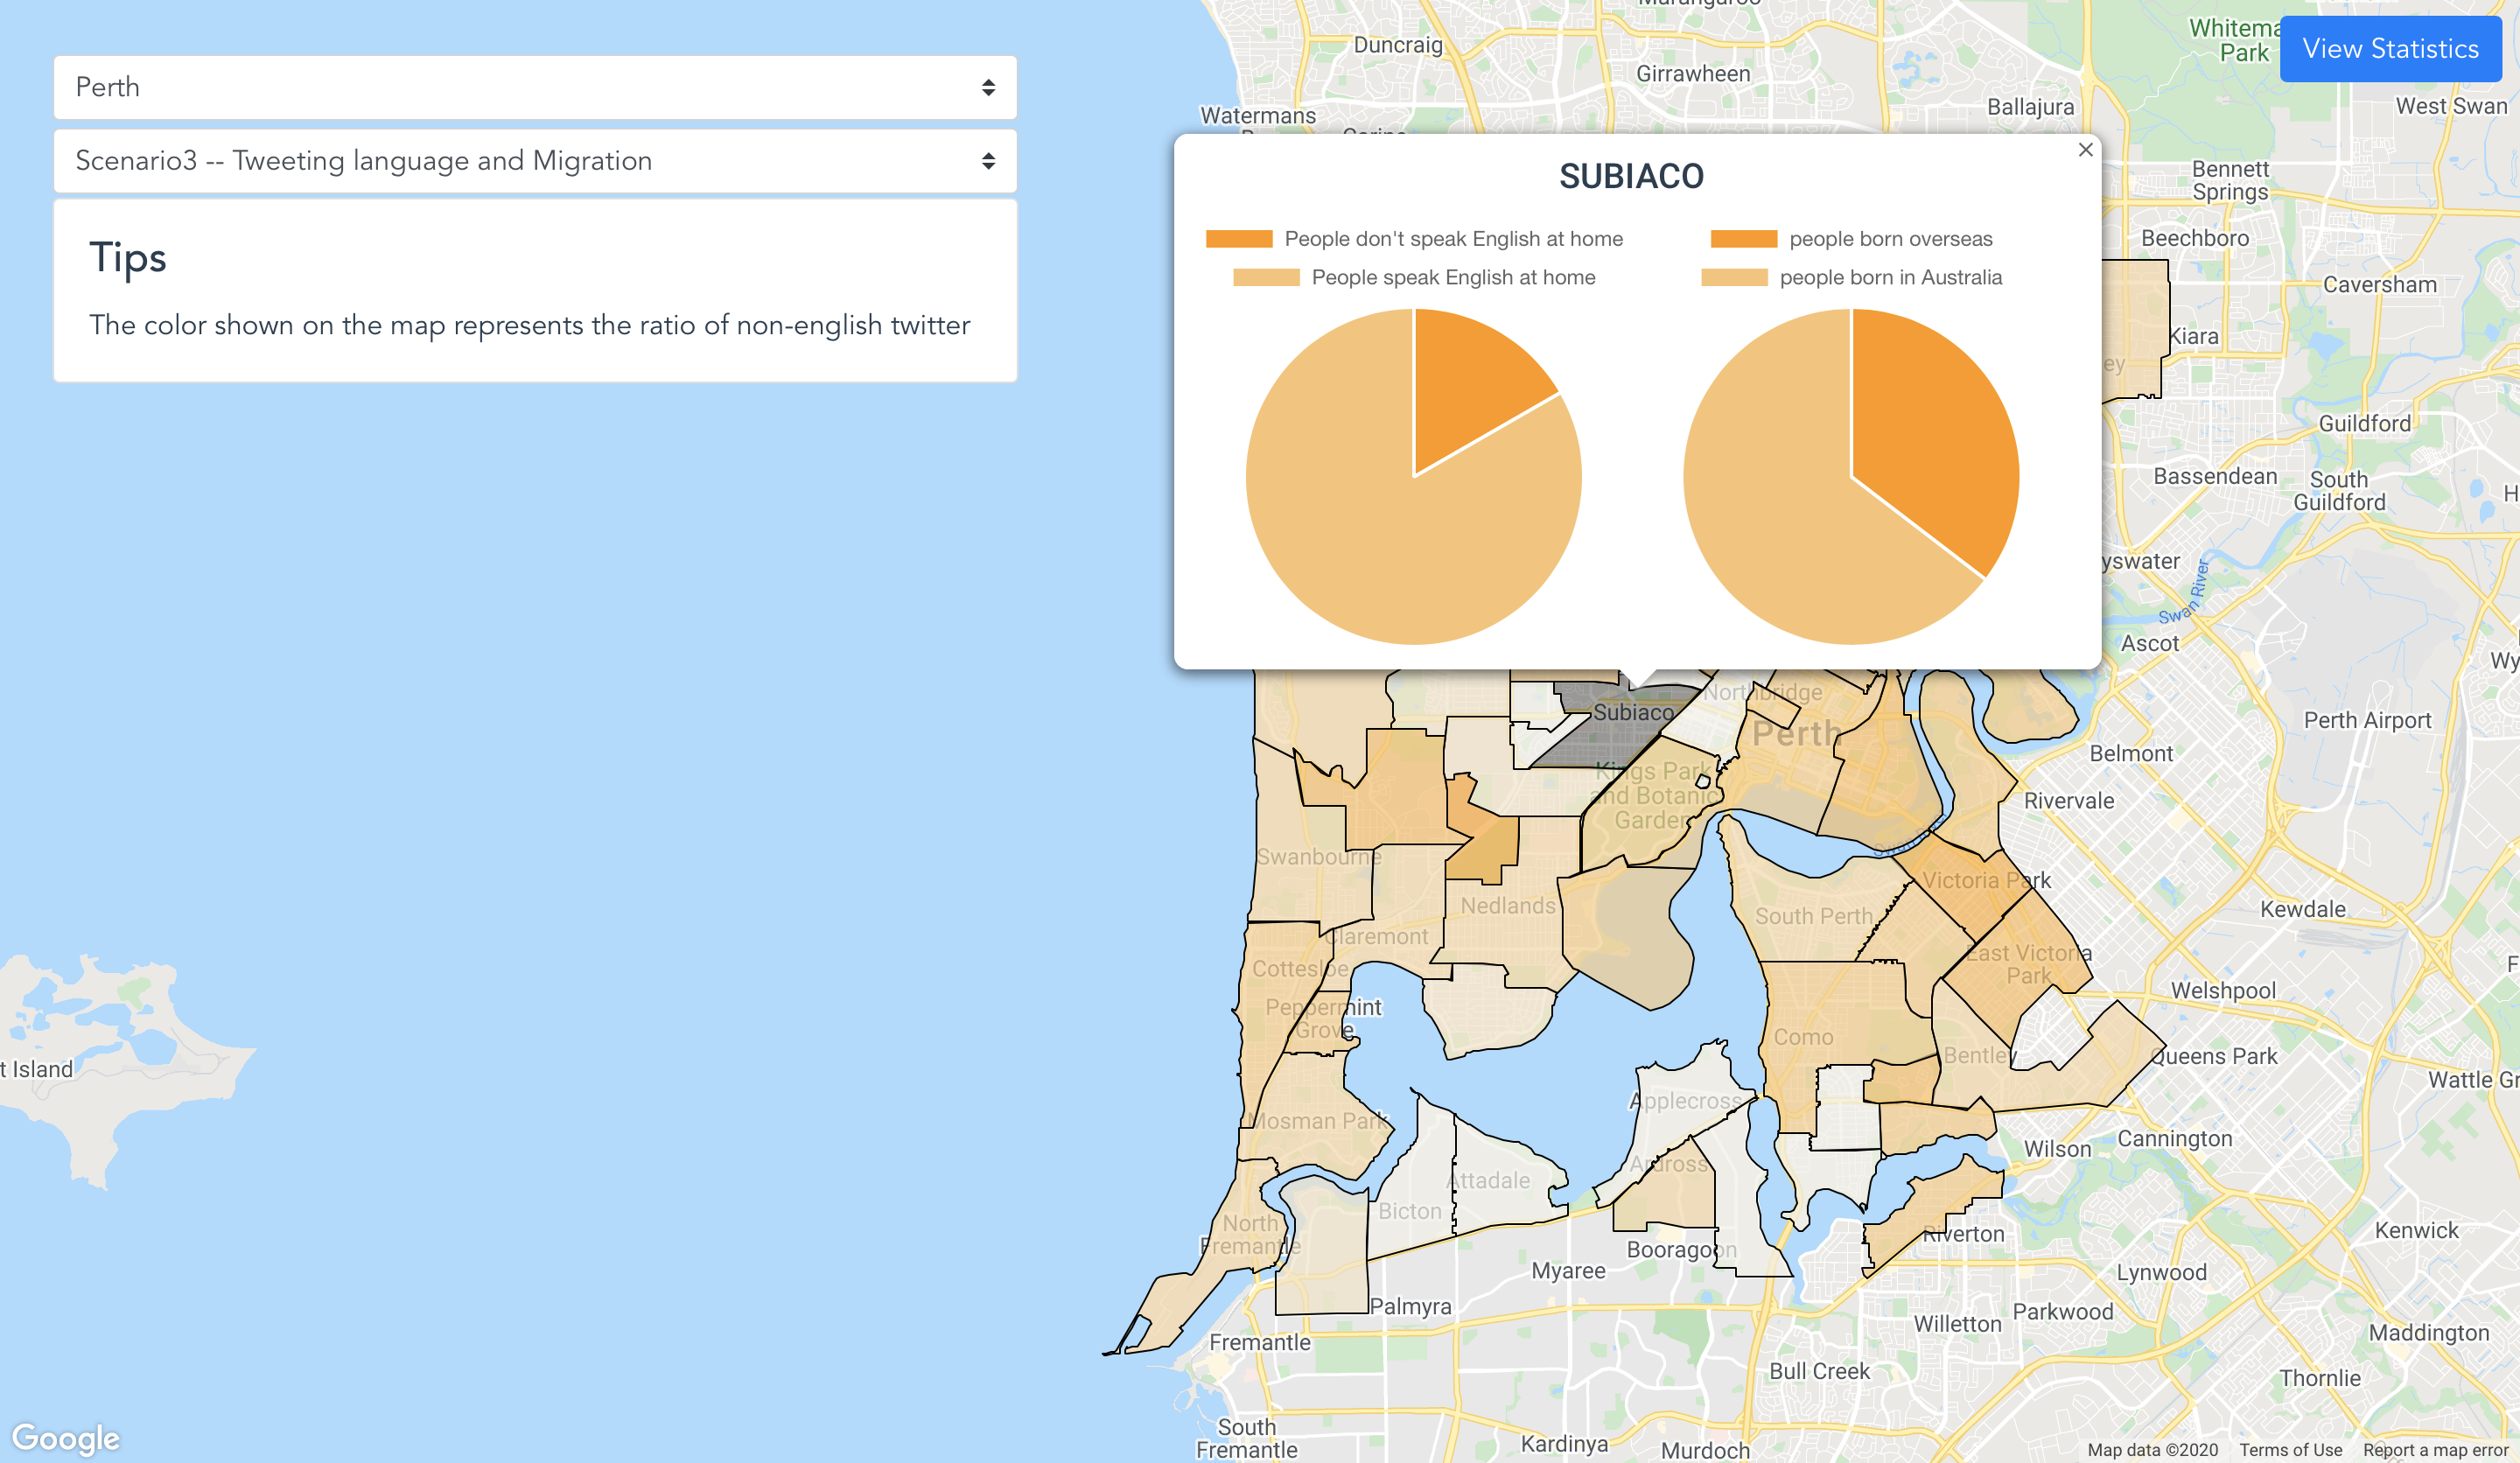
\includegraphics[width=\textwidth]{img/Perth_pie_chart.jpg}
\caption{the Pie charts in Scenario 3 for the suburb Subiaco}
\label{fig:Perth_pie_chart}
\end{figure}

\begin{figure}[htp]
\centering
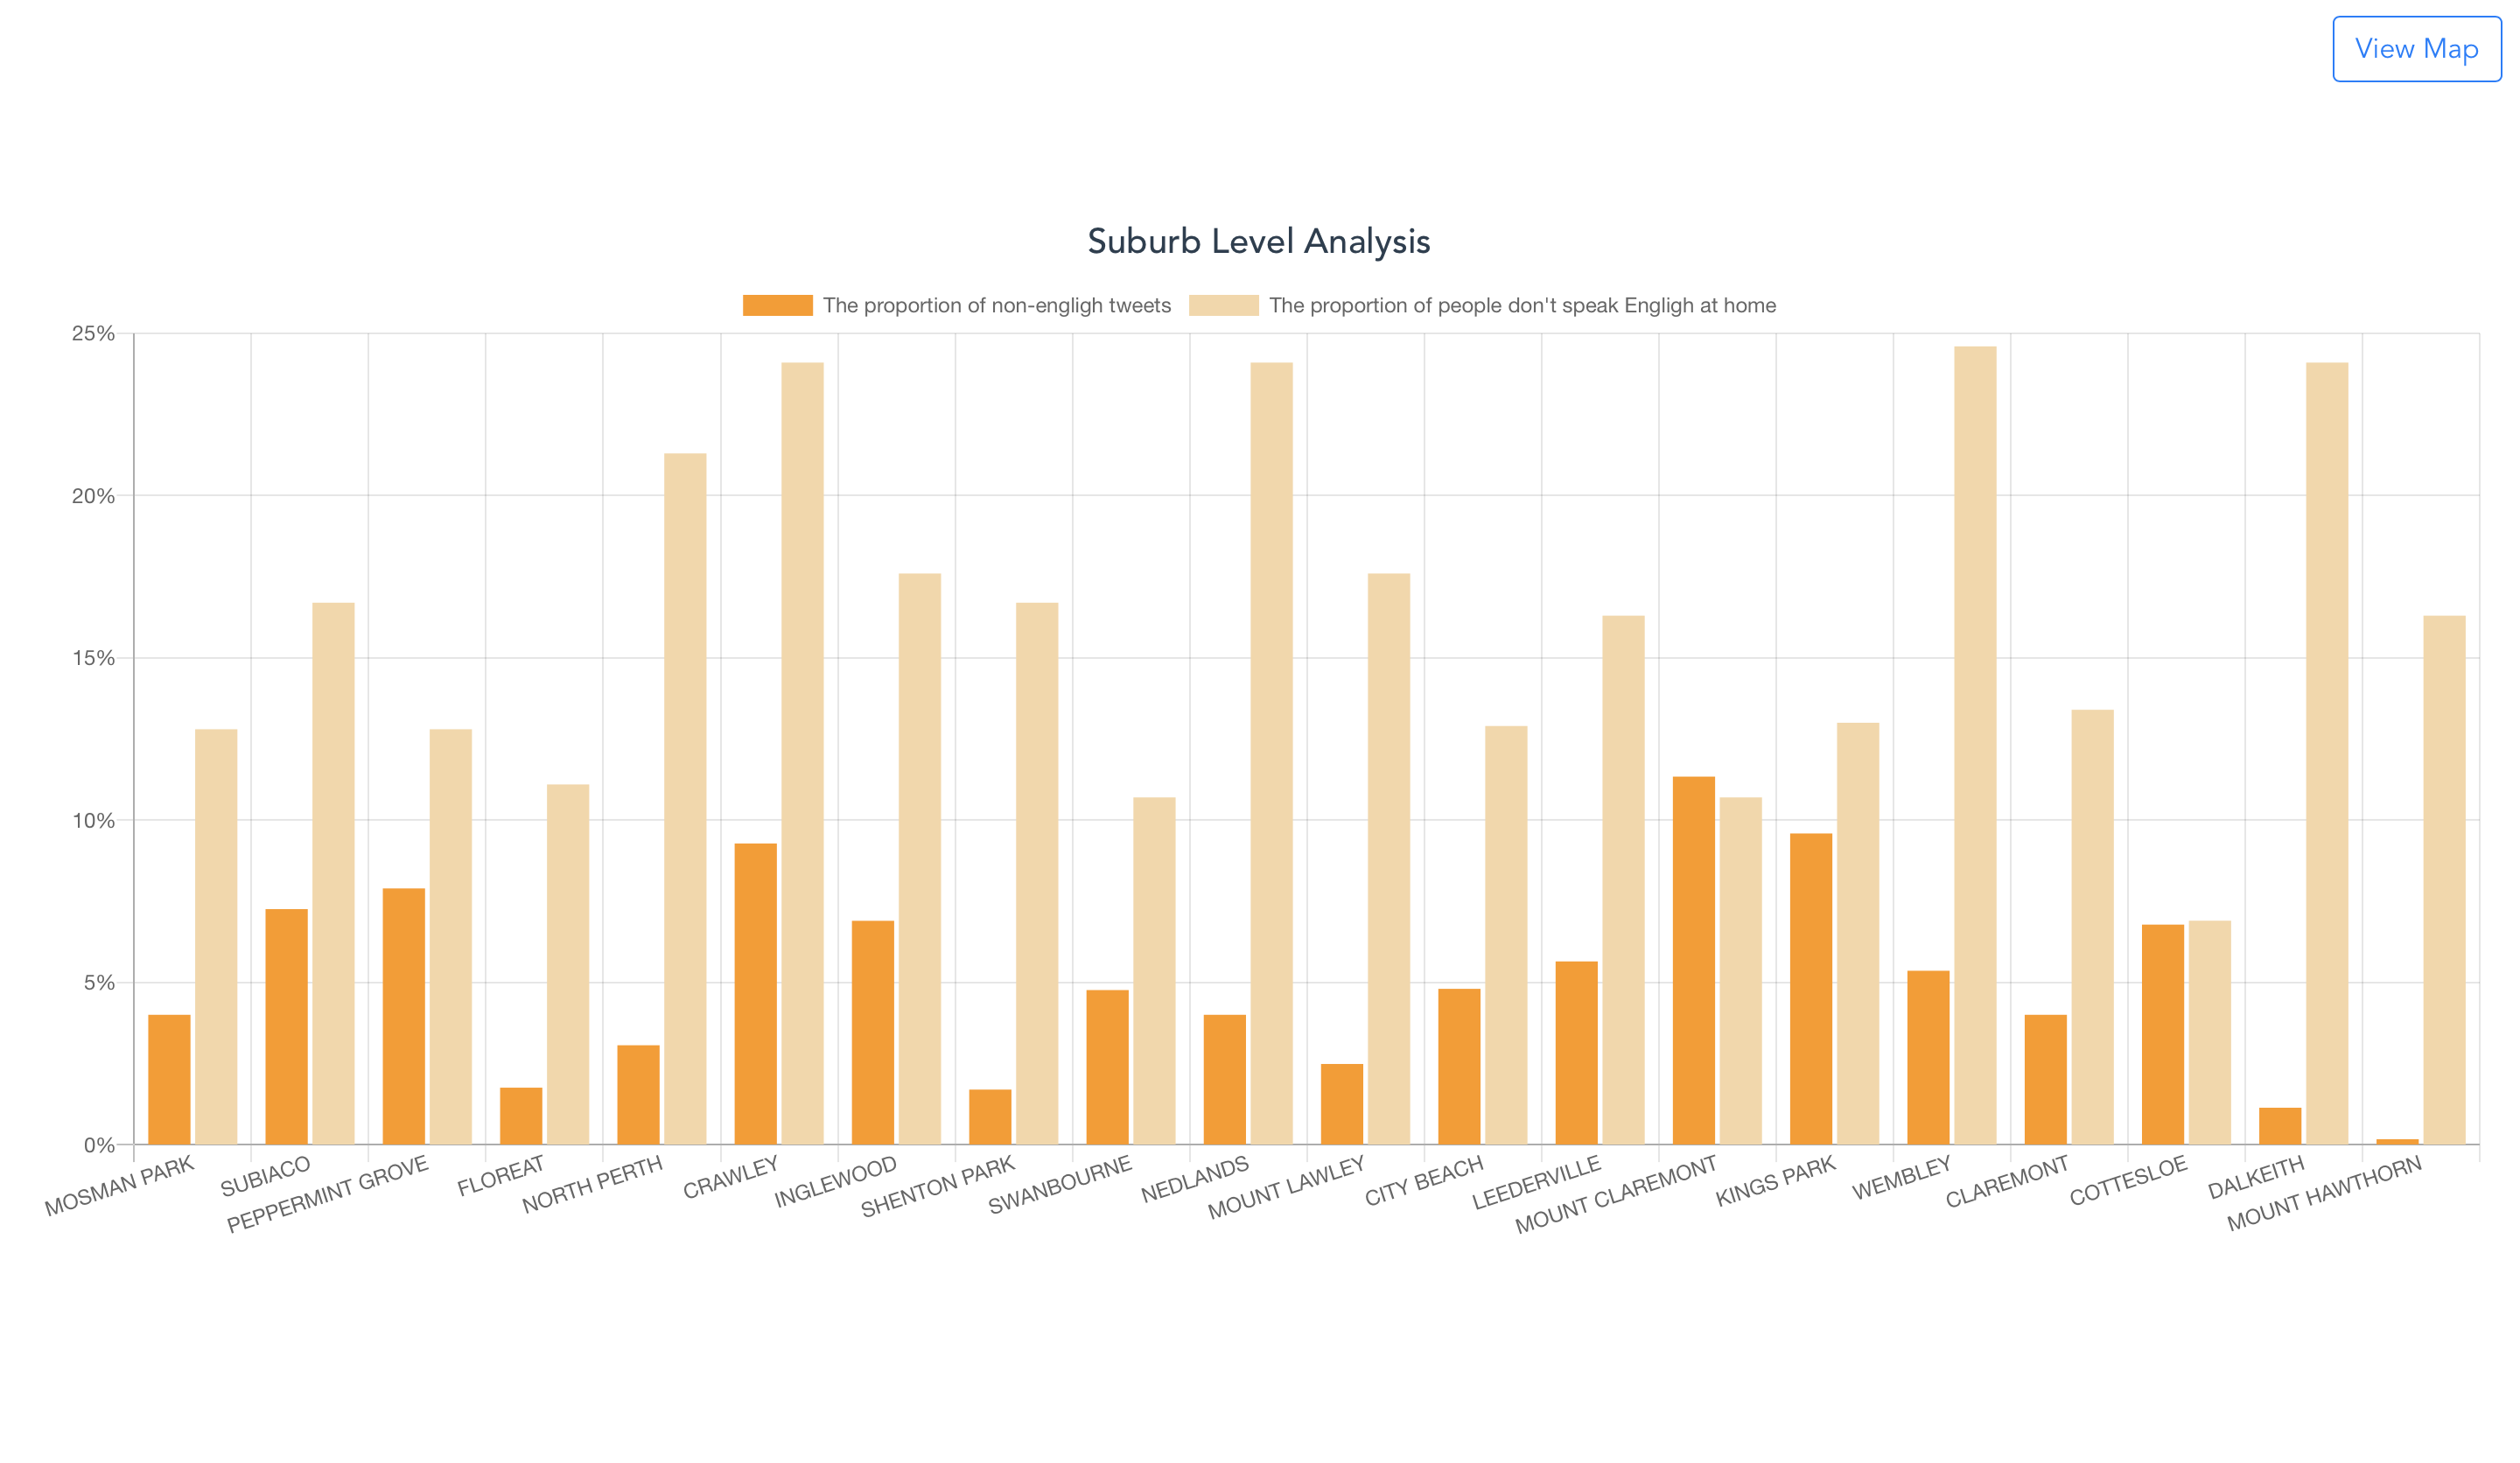
\includegraphics[width=\textwidth]{img/Perth_histogram.jpg}
\caption{the Relation between Non-English Tweets and the Proportion of people who don't speak English in Perth city}
\label{fig:Perth_histogram}
\end{figure}

\section{NeCTAR Research Cloud}

\section{User Guide}

\section{Conclusion}
In the project, an integrated cloud-based HPC system is developed on NeCTAR Research Cloud to gather and analysis tweets in Australia with five different aspects. The system has scripted deployment capabilities using Ansible. Also, it is designed with high availability and fault tolerance capability. The analysis covered five major cities in Australia and can be drilled down to suburb levels.  A web portal is provided to end users for accessing the data through ReSTful design.
\section{Team Members and Roles}
Many of the techs used in the project are quite new to our team, and thus we have been facing a lot of challenges and problems. But our teammates have done great work to study and utilize these cutting edge technologies into our system. We had good communication and proper project management to finish the development followed by a success deployment right on time. Each member has been taken a role as listed below:
\begin{table}[]
    \centering
    \begin{tabular}{l|p{13cm}}
    \hline
    Aoqi Zuo & Twitter harvester implementation, scenario designing \\
    \hline
    Rongbing Shan & Database administration, data processing, docker SWARM  \\
    \hline
    Tingli Qiu & Analyzer module implementation, scenario designing, and analysis result presentation exemplar designing \\
    \hline
    Yawei Sun & ... \\
    \hline
    Zhaofeng Qiu & ...\\
    \hline
    \end{tabular}
    \caption{Team Members and Roles}
    \label{tab:my_label}
\end{table}




%%%%%%%%%%% May be useful in the future:%%%%%%%%%%%%%%%%%%

% \begin{file}[2nodes8cores.slurm]
% \begin{lstlisting}[]
% code
% \end{lstlisting}
% \end{file}


% \begin{file}[docker service ls (brief)]
% \begin{lstlisting}[]
% NAME                         MODE                REPLICAS      
% app_\textit{nginx}_app                global              3/3           
% app_rESTful_api_server       global              3/3             
% app_tweet_analyzer           replicated          1/1             
% app_tweet_hist               replicated ˜         1/1             
% app_tweet_hist_Adelaide      replicated          1/1             
% app_tweet_hist_Brisbane      replicated          1/1             
% app_tweet_hist_Melbourne     replicated          1/1             
% app_tweet_hist_Perth         replicated          1/1             
% app_tweet_hist_Sydney        replicated          1/1             
% app_tweet_stream             replicated          1/1             
% app_tweet_stream_Adelaide    replicated          1/1             
% app_tweet_stream_Brisbane    replicated          1/1             
% app_tweet_stream_Melbourne   replicated          1/1             
% app_tweet_stream_Perth       replicated          1/1             
% app_tweet_stream_Sydney      replicated          1/1 
% \end{lstlisting}
% \end{file}

\bibliography{lib}
\end{document}
